% !TeX spellcheck = it_IT
\documentclass{beamer}

\usepackage[latin1]{inputenc}
\usepackage[tight]{subfigure}
\usepackage{graphicx}
\usepackage{multirow}
\usepackage{threeparttable}
\usepackage{booktabs}

\graphicspath {{imgs/}}
\usepackage{tikz}
\usetikzlibrary{calc,shapes,arrows,chains,shadows,arrows,fit,positioning,backgrounds,spy}
\newcommand\norm[1]{\left\lVert#1\right\rVert}
\usetheme[pageofpages=of,% String used between the current page and the
% total page count.
bullet=circle,% Use circles instead of squares for bullets.
titleline=true,% Show a line below the frame title.
alternativetitlepage=true,% Use the fancy title page.
titlepagelogo=logo_univpm.png,% Logo for the first page.
%watermark=brando1,% Watermark used in every page.
%watermarkheight=20px,% Height of the watermark.
%watermarkheightmult=5,% The watermark image is 4 times bigger
% than watermarkheight.
]{Torino}

\setbeamertemplate{background}{
	\tikz[overlay,remember picture] 
	\node[at=(current page.north east),anchor=north east,inner sep=15pt] {
\includegraphics[height=1cm, keepaspectratio]{logo_univpm_scritta.png}};
}

\author{\textbf{Studente:}Diego Droghini}
\title{Scuola di Dottorato in Ingegneria dell'Informazione}
\subtitle{XVII Ciclo n.s., 3� anno di corso (2017/2018)}
\institute{Universit� Politecnica delle Marche\\ \textbf{Progetto Eureka}}
\date{}

\definecolor{darkgray}{RGB}{50,50,50}

\setbeamercolor{section in toc}{fg=black}
\setbeamercolor{subsection in toc}{fg=darkgray}
\setbeamerfont{subsection in toc}{size=\small}
\setbeamertemplate{section in toc}[ball unnumbered] %[sections numbered]
%\setbeamertemplate{subsection in toc}[subsections numbered]


\begin{document}

\begin{frame}[t,plain]
\titlepage
\end{frame}

\begin{frame}[t]{PhD Thesis}
	\vspace{1.5cm}
	\centering
	\huge
	\textbf{Ambient Intelligence:
\\
	Computational Audio Processing
	For Human Fall Detection}
\end{frame}

%\begin{frame}{Overview}
%	\tableofcontents
%	% You might wish to add the option [pausesections]
%\end{frame}
\begin{frame}
	\frametitle{Outline}
	\begin{columns}[t]
		\begin{column}{.5\textwidth}
			\tableofcontents[sections={1-4}]
		\end{column}
		\begin{column}{.5\textwidth}
			\tableofcontents[sections={5-8}]
		\end{column}
	\end{columns}
\end{frame}

\AtBeginSubsection[]{%
	\begin{frame}<beamer>{Index}
		\tableofcontents[currentsection,currentsubsection]
	\end{frame}
}
\AtBeginSubsection[]{%
	\begin{frame}<beamer>{Index}
			\begin{columns}[t]
				\begin{column}{.5\textwidth}
					\tableofcontents[sections={1-4}, currentsection,currentsubsection]
				\end{column}
				\begin{column}{.5\textwidth}
					\tableofcontents[sections={5-8},currentsection,currentsubsection]
				\end{column}
			\end{columns}
		\end{frame}

}



\section{Introduction}	
\subsection{Fall Detection System and Challange}	
\begin{frame}{Human fall: a real problem for society}
	%			"And why do we fall, Bruce? So we can learn to pick ourselves up" cit. Batman Begins
	\begin{block}{"And why do we fall, Bruce? So we can learn to pick ourselves up" cit. Alfred - Batman Begins}
		
		\begin{itemize}
			\item 62\% of injury-related hospitalizations for the
			people over 65 years are the result of a fall \cite{gurley1996persons}
			\item main cause of death due to accidents for people
			over 65 \cite{mubashir2013survey}
			\item can lead to psychophysical repercussions on people \cite{abbate2010monitoring}
		\end{itemize}
	\end{block}
	\begin{block}{What can be done whit FCS}
		
		\begin{itemize}
			\item Monitoring of the elderly or people who live alone
			\item Assistance time reduction
		\end{itemize}
		
	\end{block}
	
\end{frame}
\begin{frame}{Fall Classification System Challenge \cite{khan2017review}}
	
	\begin{itemize}
		\item Try to collect sufficient human fall data: supervised or analytical methods
			\begin{itemize}
				\item difficulty in retrieving examples that
				represent human falls
			\end{itemize}	

		\item Deal with no human fall data: Novelty detection approach
			\begin{itemize}
				\item good description of "normality"
				
		\end{itemize}
	\end{itemize}
	
	
	\begin{minipage}[c]{0.48\textwidth}
		
		\begin{block}{Related Work}	
			\begin{itemize}
				\item Wearable
				\begin{itemize}
					\item \textbf{Accelerometers}
					\item Gyroscopes 	
				\end{itemize}
				\item Ambient 
				\begin{itemize}
					\item \textbf{Vision System}
					\item Audio microphone
					\item Radar doppler 	
				\end{itemize}				
			\end{itemize}
		\end{block}
		
	\end{minipage}
	\hfill%
	\begin{minipage}[c]{0.48\textwidth}
		\begin{block}{Issues}
			\begin{itemize}
				\item no standard datasets;
				\item no standard methodology
				\item difficult comparison with other methods;
				\item no audio dataset available
				\item scarcity of real human falls
			\end{itemize}
		\end{block}
%		\centering
%		\hspace{0.8cm}\alert{Fall Event} \\
%		\vspace{0.5cm}
%		\hspace{0.8cm}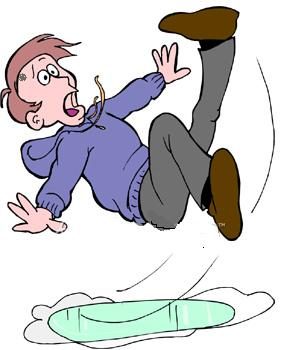
\includegraphics[width=0.5\textwidth]{imgs/slip_and_fall}\\
		
	\end{minipage}%
\end{frame}

\subsection{Motivations and Contributions}	
\begin{frame}[t]{Motivations and Contributions}
	\footnotesize
	\begin{minipage}[t]{0.45\textwidth}
		Analytical methods:
		\begin{itemize}
			\item exploiting some a priori knowledge;
			\item manual tuning of the hyperparameters;
			\item applying a threshold on aquired signals or features;
		\end{itemize}
		 They can hardly perform when the operating conditions and the subjects are variable.
  	\end{minipage}
	  \hfill
 	\begin{minipage}[t]{0.45\textwidth}
	Machine learning methods:
	\begin{itemize}
		\item learns from the data;
		\item can be eforced by exploiting some a priori knowledge;
		\item no need of manual tuning of the hyperparameters;
	\end{itemize}
	\vspace{0.4cm}
	They need more data!
 	\end{minipage}
 	\begin{block}{Contributions}
		\begin{itemize}
			\item audio based fall detection is a reliable alternative;
			\item proposal and evaluation of the FD task dedicated FAS sensor;
			\item proposal of the acoustic A3FALL dataset to the community.
		\end{itemize}
 	\end{block}
%	and the subjects are variable
%	analytical methods distinguish between fall and nonfall events by applying a threshold directly on the acquired signals or on the
%	features sequences extracted from them. These methods are generally built
%	exploitin in a specific scenario g some a priori knowledge to operateand needs
%	manual tuning of the hyperparameters of the algorithm. For these reasons,
%	the ?analytical methods? can hardly perform when the operating conditions
%	and the subjects are variable. In ?machine learning? methods, the algorithm
%	learns from the data how to discriminate falls from non-falls.
%	The main contribution is to demonstrate that the audio human fall detection is a reliable
%	solution and not only the mainstream systems based on vision or wearable sensors can be used for this kind of problem. A particular acoustic sensor specially
%	designed for the fall detection task is proposed and evaluated. Moreover, the
%	dataset used to assess all the proposed methods has been created by the same
%	authors and made available by the scientific community
	
\end{frame}

\section{Dataset}
\subsection{FAS}
		\begin{frame}{Floor Acoustic Sensor\cite{Principi2016a}}%\footnotemark}
	
	\begin{minipage}[c]{0.5\textwidth}
		\begin{enumerate}
			\item The outer container
			\item The inner container
			\item The microphone slot
			\item The membrane touching the floor
		\end{enumerate}
	\end{minipage}%
	\hfill%
	\begin{minipage}[c]{0.5\textwidth}
		\centering
		
		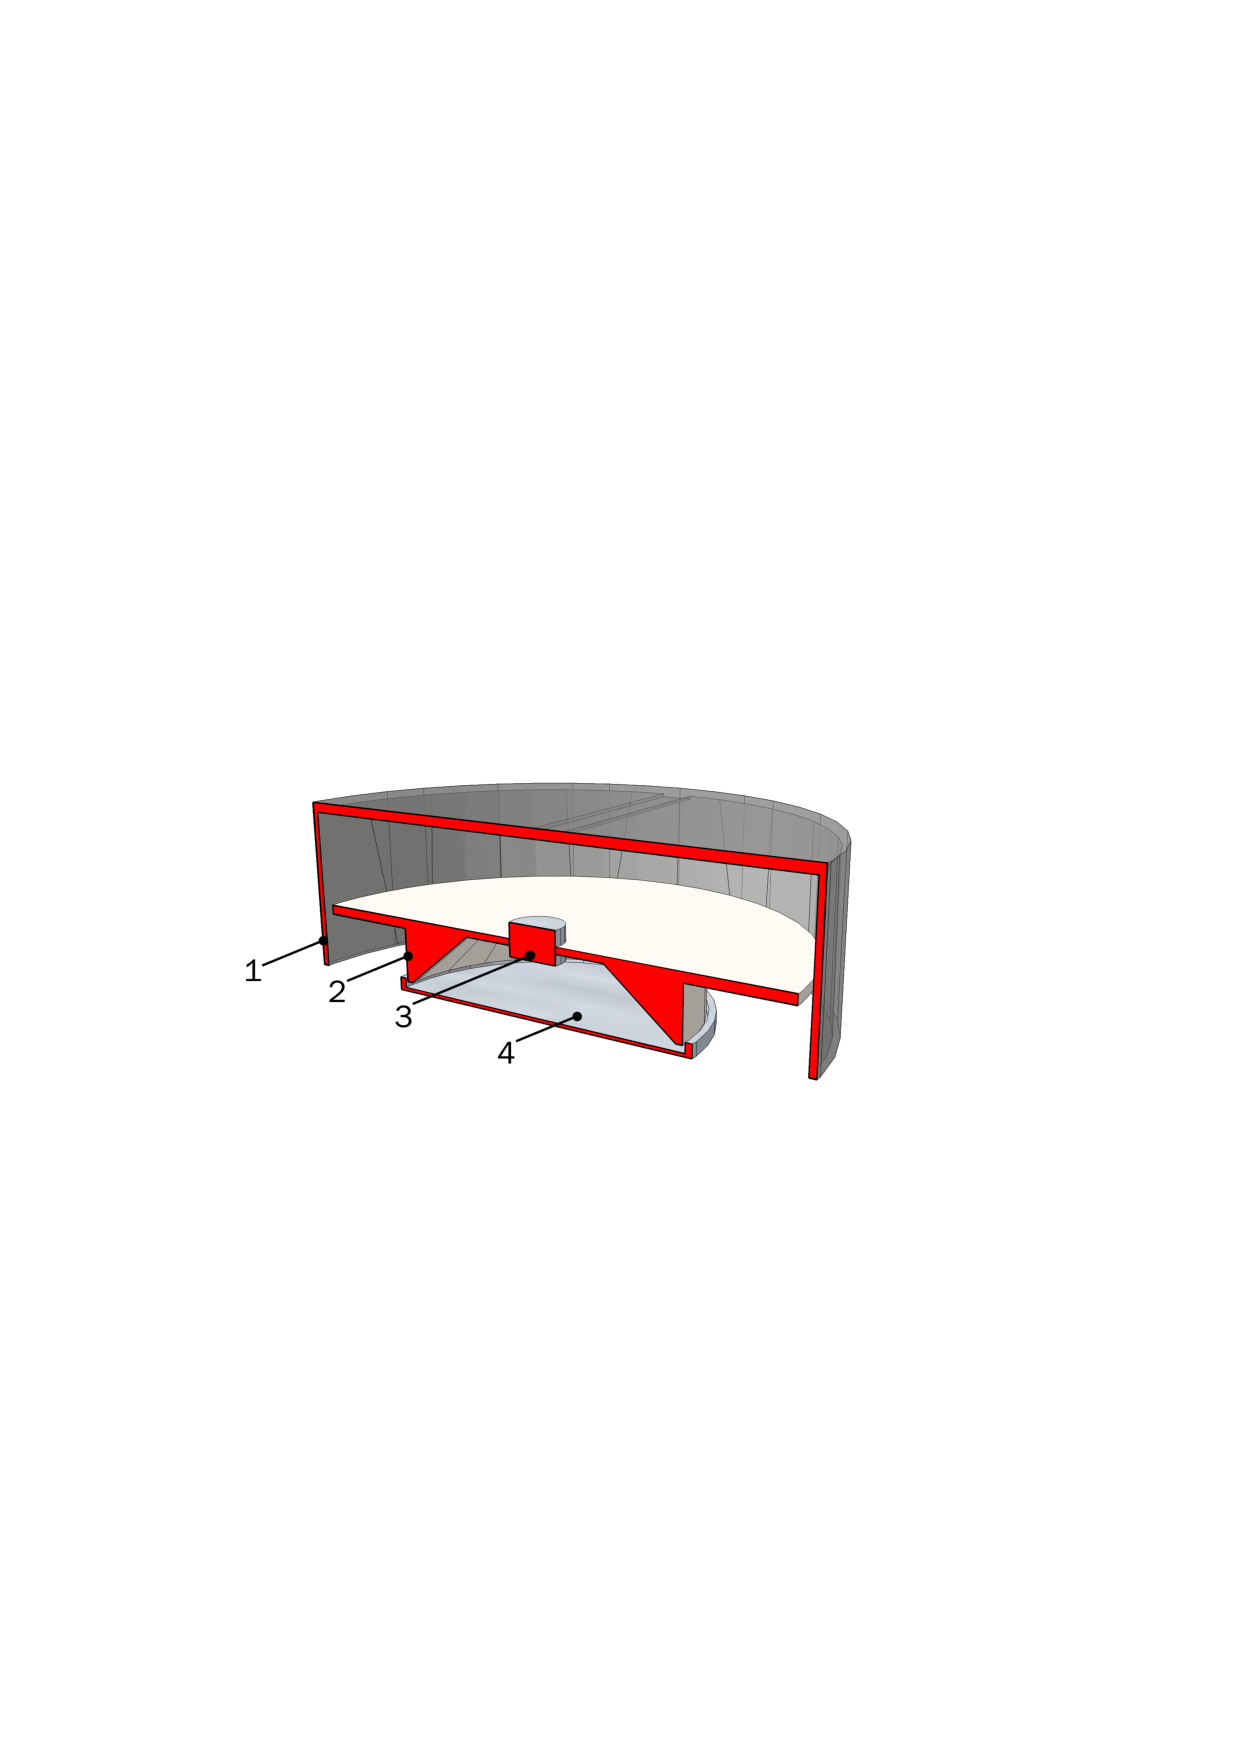
\includegraphics[width=1\textwidth]{imgs/AcousticSensor}\\
		
	\end{minipage} 
	\begin{block}{Advantage}
		\begin{itemize}
			\item Easily integrated into the environment
			\item More sensitive to signals related to falls
		\end{itemize}
	\end{block}
	%\vspace{0.5cm}
	\begin{columns}[c]
		\begin{column}[c]{0.5\textwidth}
			\hspace{1.5cm}\vspace{0.2cm}
			3D printed prototype 	
		\end{column}
		\begin{column}[c]{0.5\textwidth}
			\hspace{1cm}\vspace{.2cm}				
			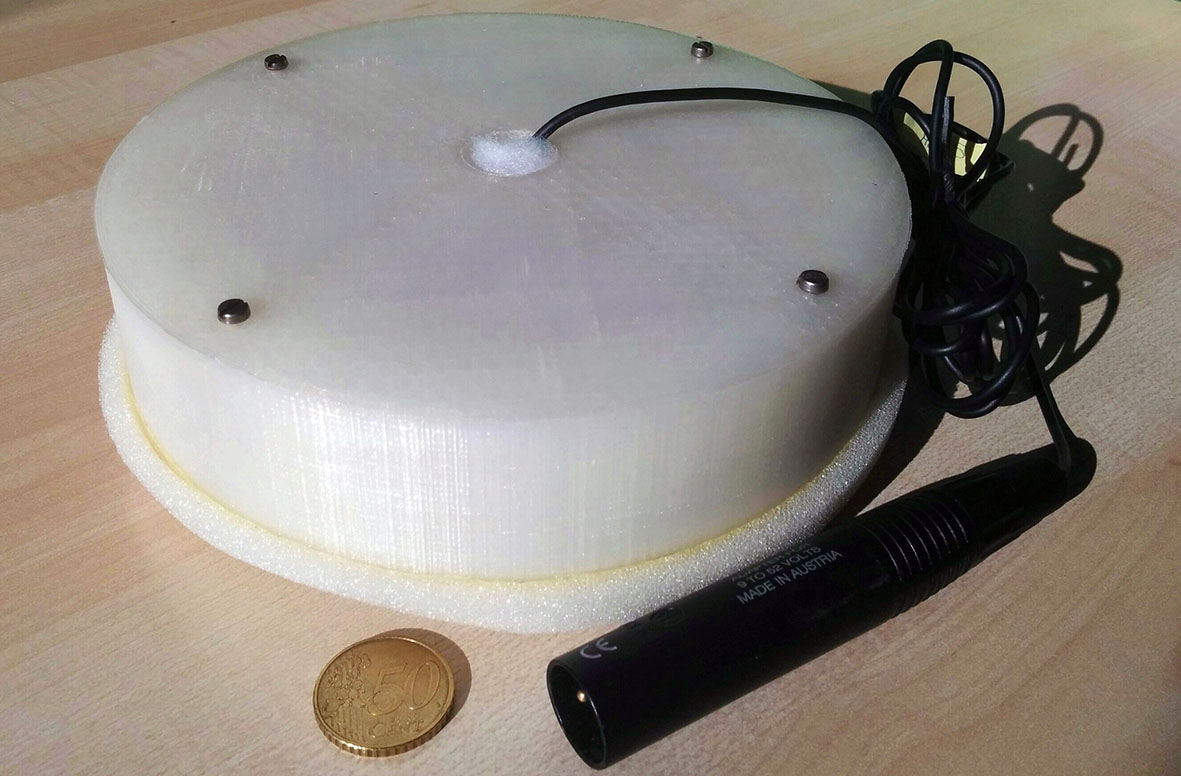
\includegraphics[width=0.6\textwidth]{imgs/FAS_front_little.jpg}
		\end{column}
	\end{columns}
	
	%\footnotetext[1]{Patent AN2013A000056, 18/03/2013, Paolo Olivetti}
\end{frame}
	
	

\subsection{A3FALL Dataset}
\begin{frame}[t]{The fall events dataset: A3Fall}
	
	%motivazione: mancaza di dataset audio adeguati
	%descrizione generale: descrizione 3 stanze 
%	\begin{block}{Motivation}
%		\begin{itemize}
%			\item The lack of available audio datasets;
%			\item Use of the dedicated FAS sensor.
%		\end{itemize}
%	
%	\end{block}
	\begin{block}{Recording Rooms}
		\begin{itemize}
			\item R0 - rectangular room particularly suitable for the propagation of acoustic waves through the floor;
			\item R1 - university auditorium room in which the flooring is composed of fitted carpet;
			\item R2 - a recording studio
			\begin{itemize}
				\item sensors placed in the live room;
				\item audio events performed in the control room.
			\end{itemize}
			
		\end{itemize}
	\end{block}
\end{frame}


\begin{frame}[t]{Recording set-up}
%			strumentazione: microfoni (fas e aerei + randy + sceda audio + marche microfoni)
	\vspace*{-2em}
	\begin{columns}[t]
		
		\centering
		\begin{column}{0.3\textwidth}
			\begin{block}{Sampling}
				\begin{itemize}
					\item Sample Rate: 44.1 kHz
					\item Bit-depth: \\24 bit
				\end{itemize}
			\end{block}
			
			%				\centering	
			\vspace{0.5cm}
			Used sensors:
			\begin{itemize}
				\item Mic. array (3)\footnotemark[1]
				\item FAS v1\footnotemark[1]
				\item FAS v2\footnotemark	
			\end{itemize}
			%				{\small	The microphone used in both sensors:\\ \emph{AKG C400 BL}}
		\end{column}
		
		\begin{column}{0.7\textwidth}	
			\begin{block}{The recording room}
				%					\vspace{0.2cm}
				\centering
				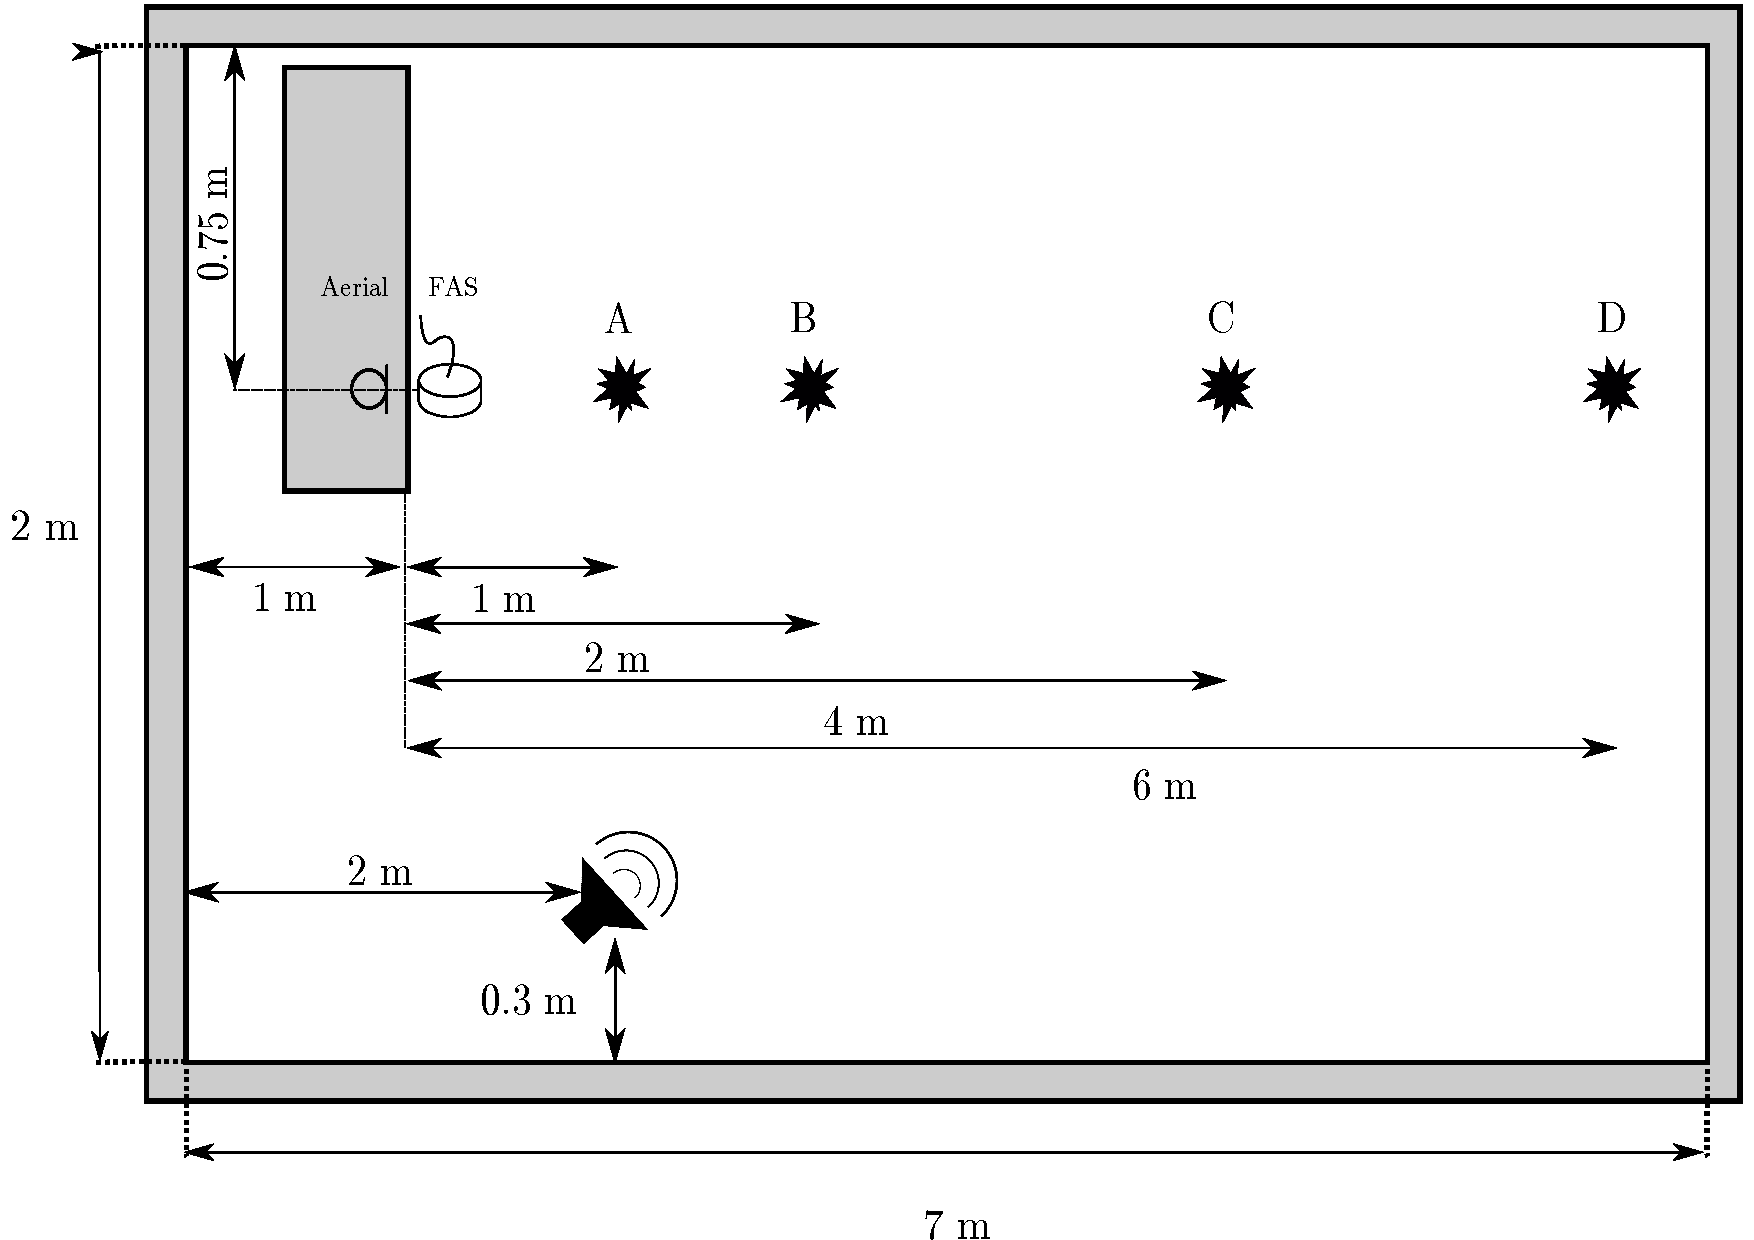
\includegraphics[width=\textwidth]{imgs/room_experiments_one_aerial.pdf}
				%\\The letters A, B, C and D indicate the positions of fall events
				
			\end{block}
			
		\end{column}
	\end{columns}
	\footnotetext[1]{AKG C400 BLT.}
	\footnotetext[2]{RODE Lavalier.}
\end{frame}

\begin{frame}[t]{Description}
%	aggingere qualcosa sulla sinistra
	\vspace*{-1cm}
	\begin{columns}[t]
		\begin{column}{0.5\textwidth}
			\scriptsize
			\begin{table}[t]
			%	\caption{Composition of the A3Fall-v2.0 dataset.}
				\label{tab:numDataset}
		
				\begin{tabular}[t]{c|ccc}
					
					\hline
					\textbf{Class} & \textbf{R0} & \textbf{R1} & \textbf{R2} \\ %\cline{2-5} 
					%& \hspace{8pt}Clean\hspace{8pt}  & \hspace{6pt}Clean\hspace{6pt}   \\ 
					\hline
					&\multicolumn{3}{c}{Nr. of occurrences}\\
					Basket      			& 64    &   40 	&   40    	\\
					Fork        			& 64    &   40 	&   40     	\\
					Ball       				& 64    &   40	&   40    	\\
					Book        			& 64    &   40	&   40    	\\
					Bag         			& 64    &   30 	&   40    	\\
					Chair       			& 96    &   40 	&   40    	\\
					Table       			& 0   	&   40 	&   40    	\\
					Guitar Slide       		& 0   	&   40 	&   40    	\\
					Nipper       			& 0    	&   40 	&   40    	\\
					Keys       				& 0    	&   40 	&   40    	\\
					Hook       				& 0    	&   40 	&   40    	\\
					Coat Hook       		& 0    	&   40 	&   40    	\\
					$\,$ Manikin Doll $\,$ 	& 44    &   0 	&   0    	\\
					$\,$ Human Fall $\,$ 	& 0    	&   40 	&   40    	\\
					\hline
					&\multicolumn{3}{c}{Total length (s)}\\			
					%			Human Activity  		& 1135  &   3050&   580   	\\
					%			Music					& 1395  &	4330&   3345  	\\
					%			Television				& 0   	&	1675&   1625  	\\
					Background  			& 2530  &   9055&   5550   	\\
					\hline
				\end{tabular}
			\end{table}
		\end{column}
		\begin{column}{0.5\textwidth}
			\begin{figure}[htb]
				\centering
				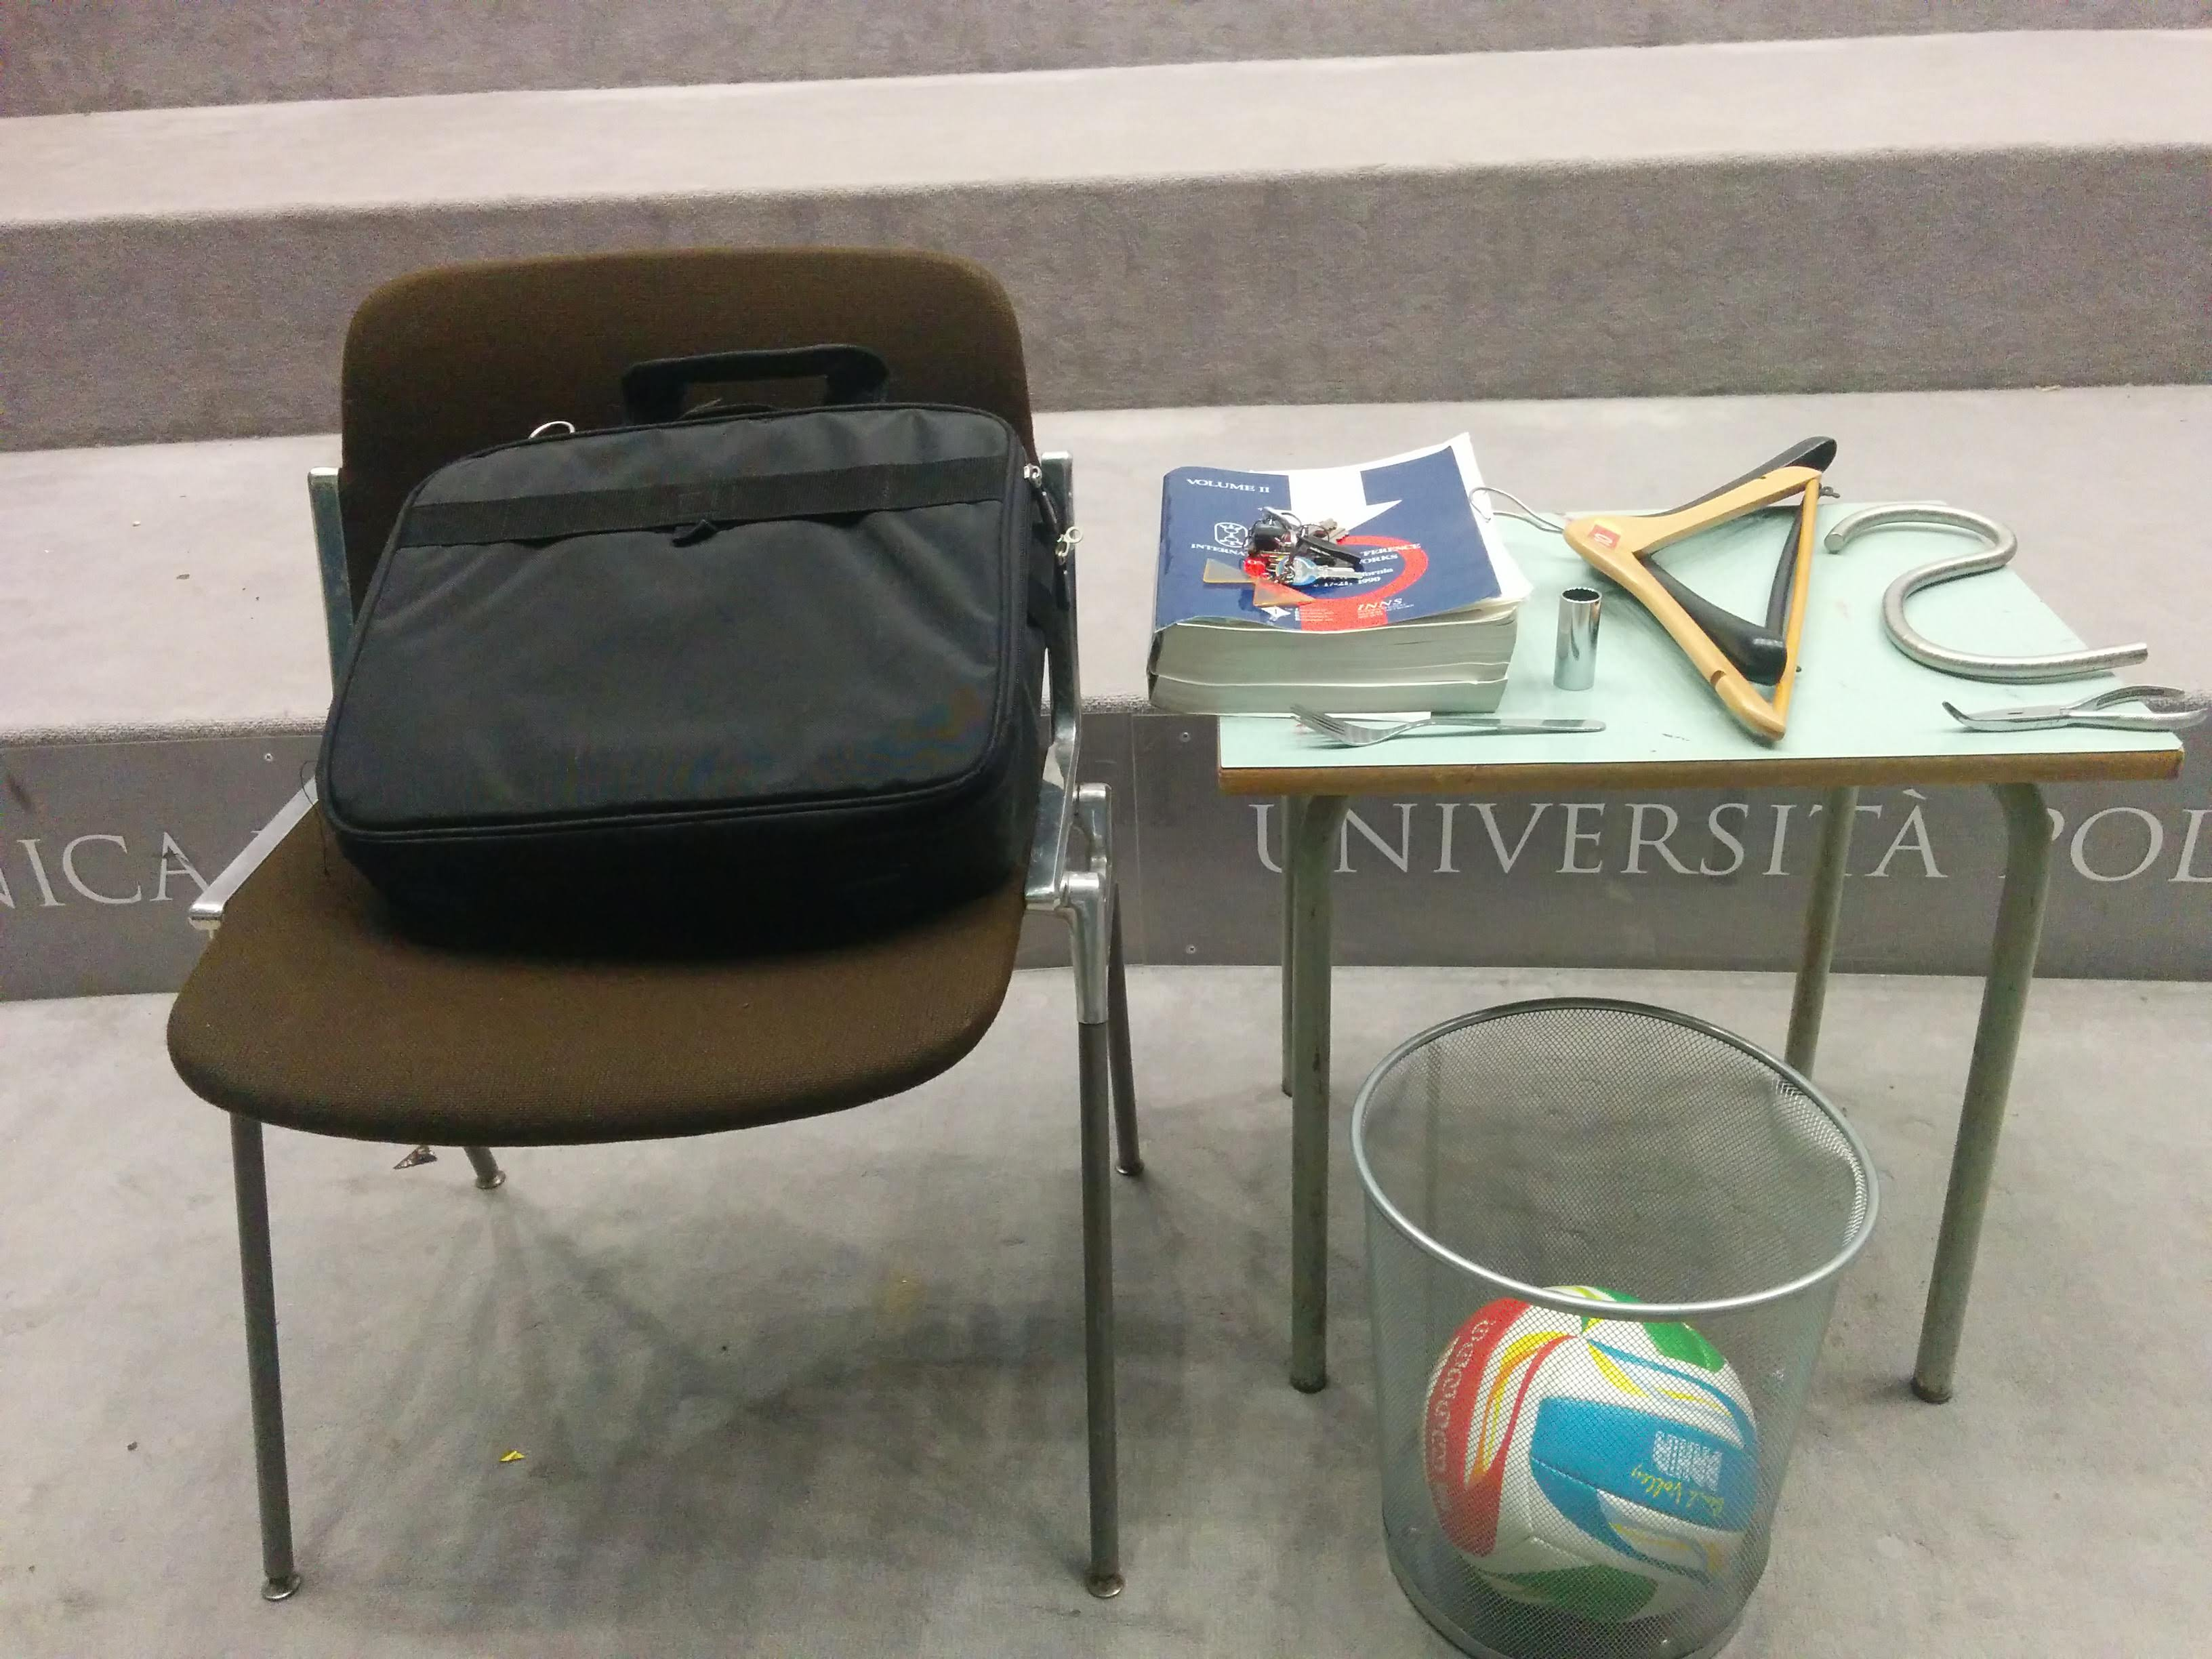
\includegraphics[height=3cm]{imgs/objects_R1_R2.jpg}\\
%				\caption{Objects employed for creating the fall events dataset.}\label{fig:objects}
			\end{figure}
			\vspace{-0.7cm}
			\begin{figure}[htb]
				\centering
				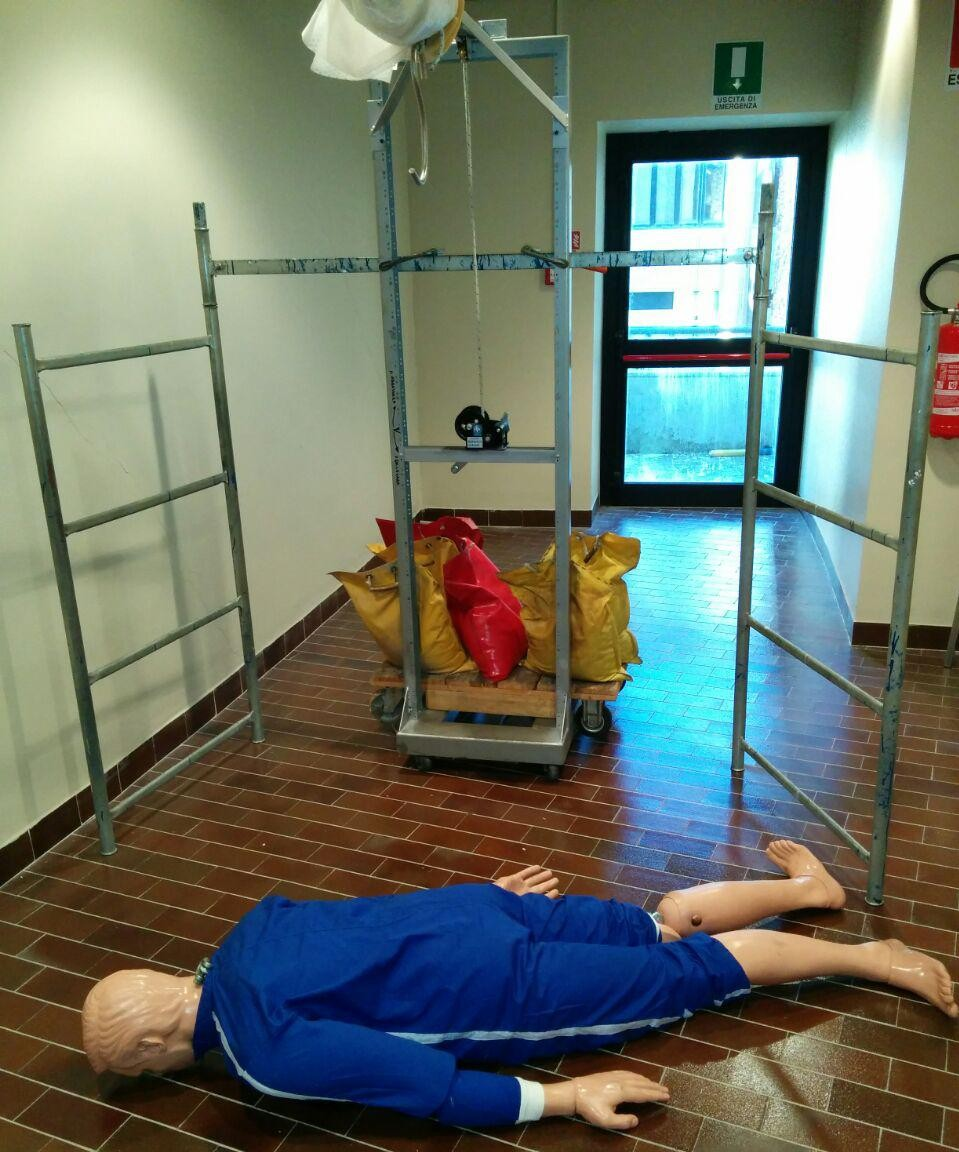
\includegraphics[height=4cm]{imgs/impalcatura}
				%				\caption{Objects employed for creating the fall events dataset.}\label{fig:objects}
			\end{figure}
		\end{column}
	\end{columns}
\end{frame}

		\begin{frame}[t]{Signals analysis}	
	\begin{columns}[t]
		\begin{column}{0.5\textwidth}
			\vspace{0.45cm}
			\centering
			Average value of the mel channels
			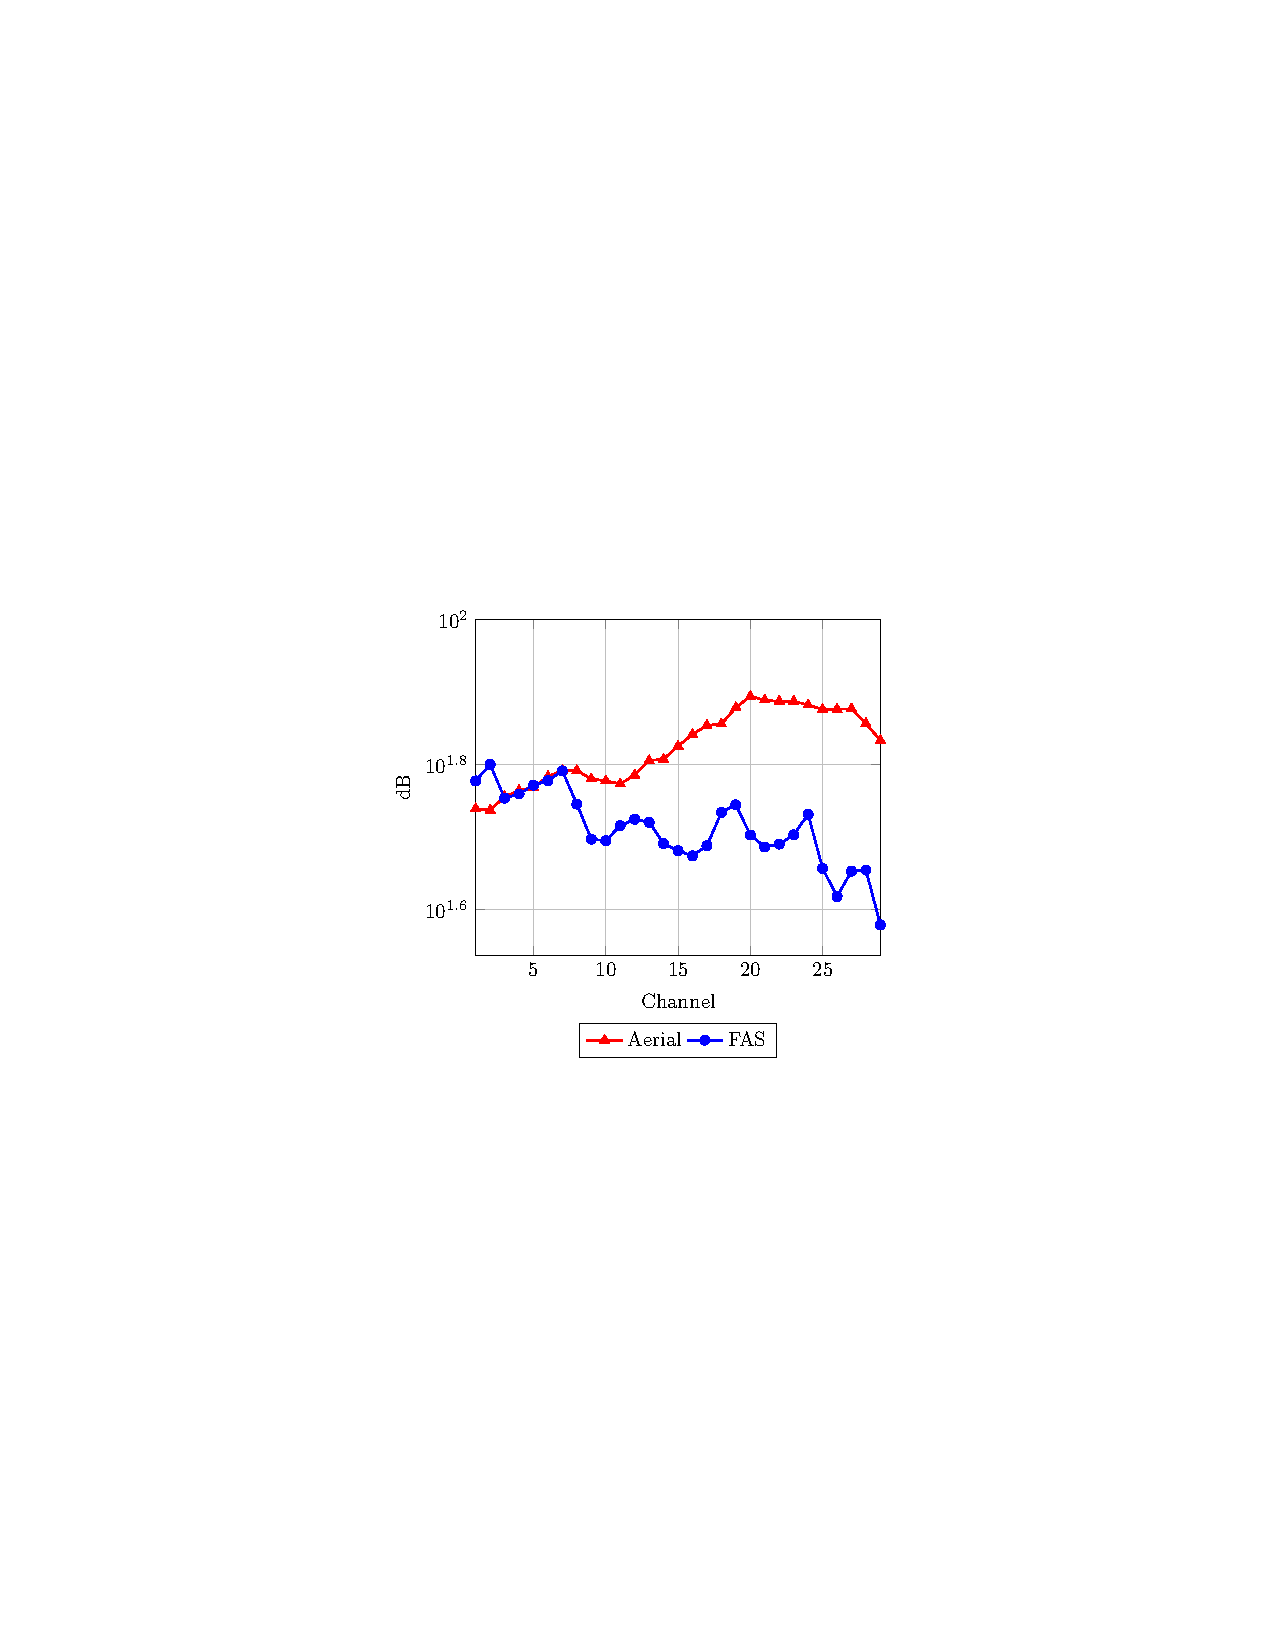
\includegraphics[width=\textwidth,height=0.7\textwidth]{imgs/mel_dB.pdf}
			
		\end{column}
		\begin{column}{0.5\textwidth}
			\centering
			Average value of the SNR for each mel channel
			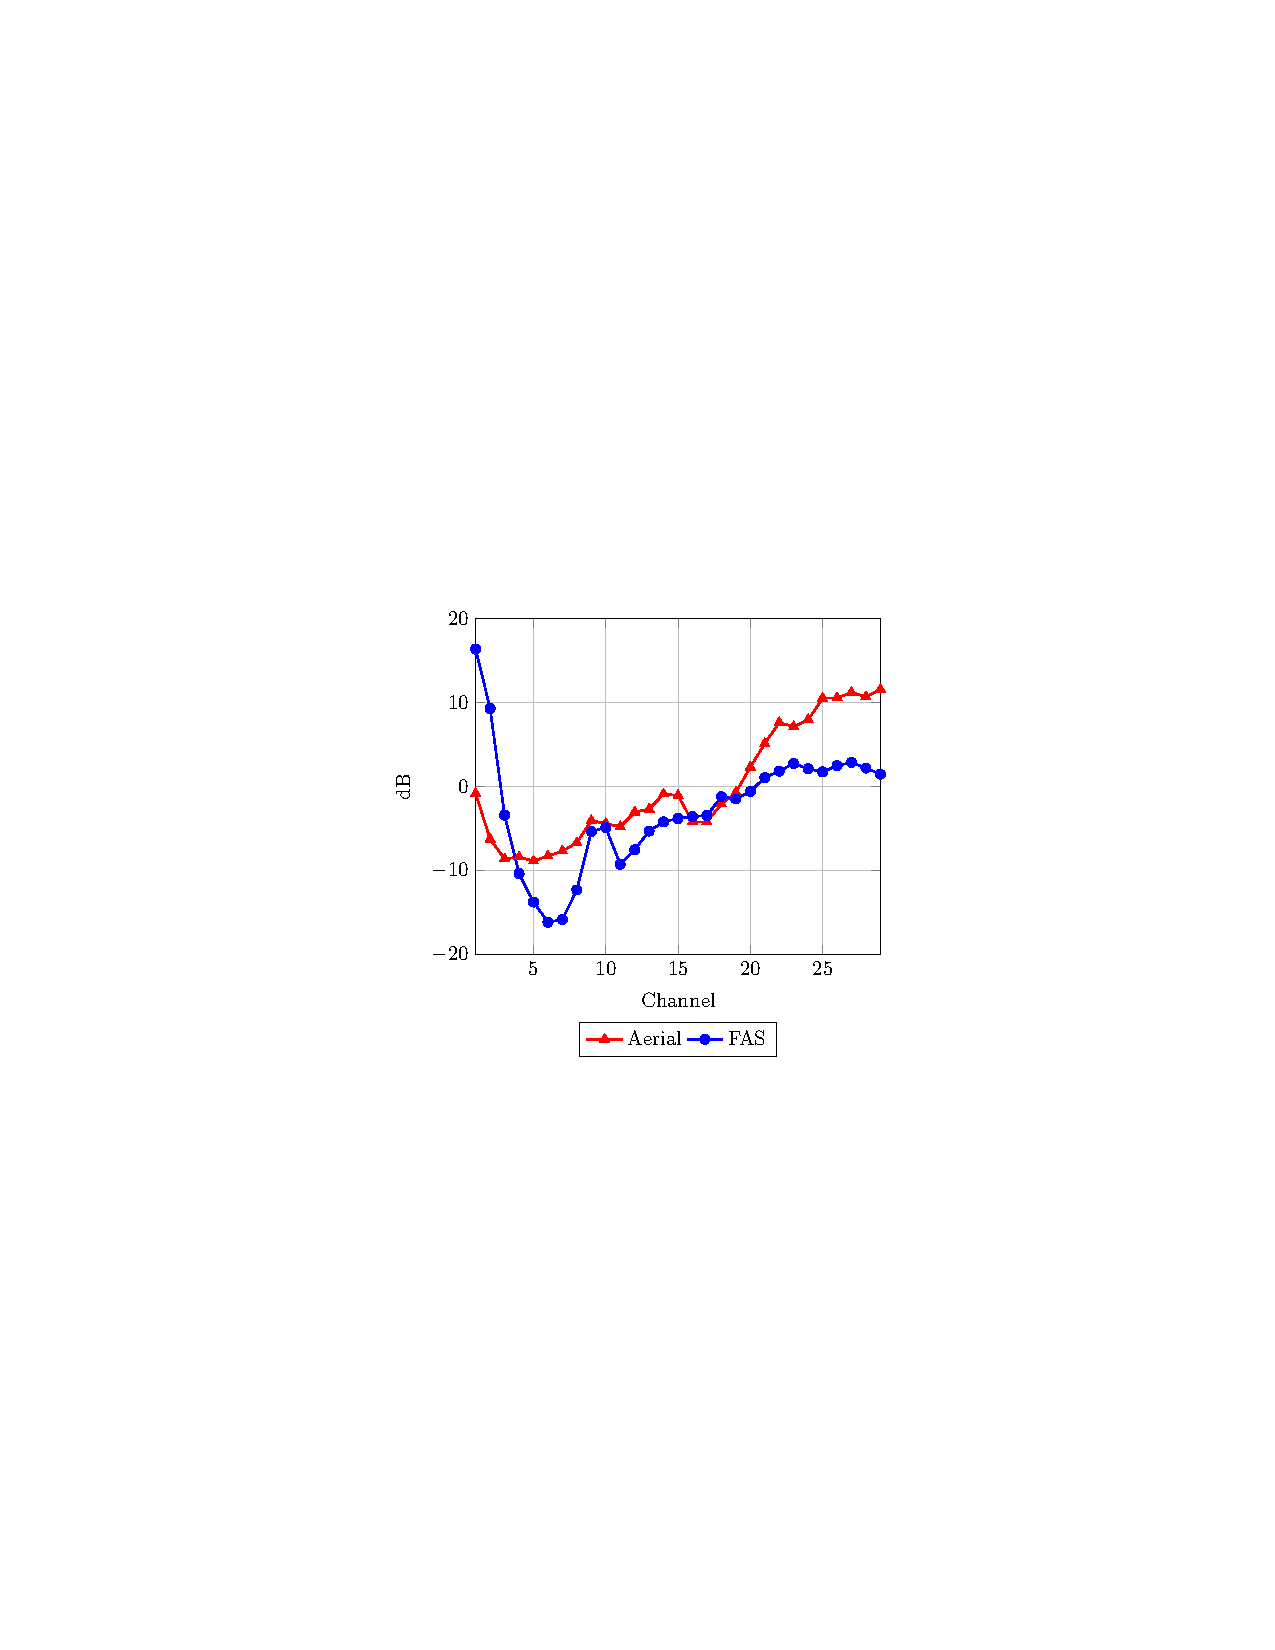
\includegraphics[width=\textwidth,height=0.7\textwidth]{imgs/SNR_mel_channel.pdf}	
			
		\end{column}			
	\end{columns}
	\begin{block}{Remark}
		\begin{itemize}
			\item The ``valley'' in the curves is due to the pitch of the music signal
			\item The FAS is better at low frequencies 
		\end{itemize}
	\end{block}	
\end{frame}
\section{Supervised Approaches}
%\subsection{Multi-class SVM}
%\subsection{Binary SVM}
\begin{frame}[t]{Supervised Approaches: SVM based}
	\begin{columns}[T] % align columns
		\begin{column}{.55\textwidth}
			%	\includegraphics[width=\textwidth]{Images/CIN_2016_approccioComplessivo}
			\begin{itemize}
				\item Completely supervised scenario
				\item GMM to model a UBM with EM algorithm
				\item MFCC features to Supervectors (MAP)
				\item SVM classificator
			\end{itemize}
			\begin{figure}
				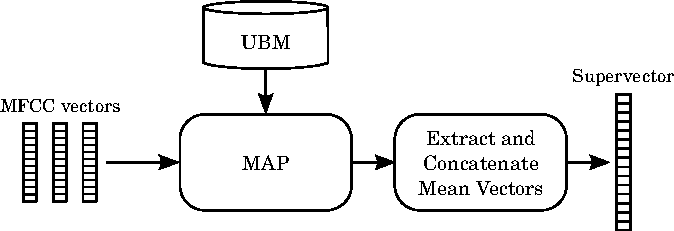
\includegraphics[width=0.8\textwidth]{imgs/gms_bn.pdf}\\
			\end{figure}
		\end{column}%
		
		\begin{column}{.35\textwidth}
			
			\centering
			\begin{figure}
				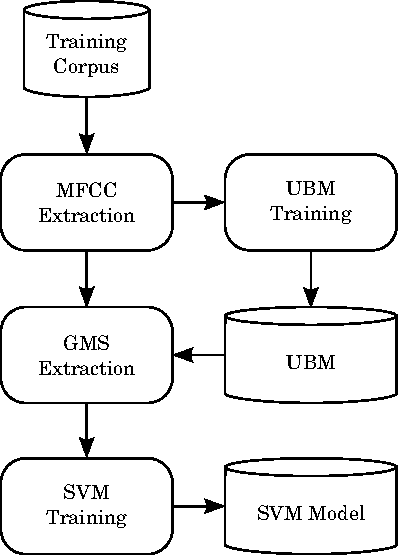
\includegraphics[width=0.8\textwidth]{imgs/training_scheme.pdf}\\
			\end{figure}
			
		\end{column}%
	\end{columns}
\end{frame}
\begin{frame}[t]{Scenarios}
		\begin{columns}[T] % align columns
		\begin{column}{.5\textwidth}
			\begin{block}{Multi-class}
			 Trained to discriminate the type of the fallen object
			\begin{figure}
				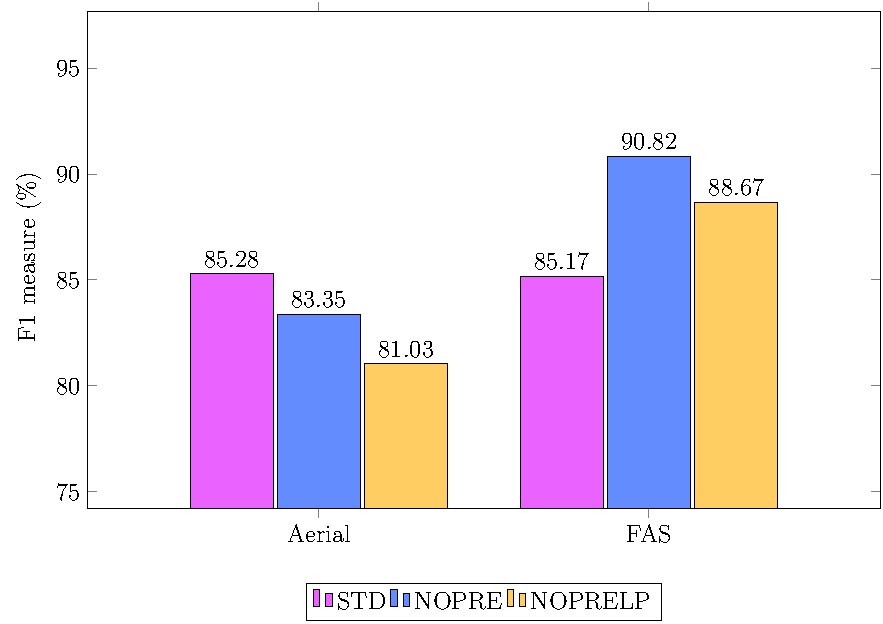
\includegraphics[width=0.8\textwidth]{imgs/16_multicondition.pdf}
			\end{figure}
			\end{block}
		\end{column}%
		
		\begin{column}{.5\textwidth}
			
			\begin{block}{Bi-class}
			Trained to discriminate fall from non-fall % testset con aggiunta di human activity noise
			\begin{figure}
				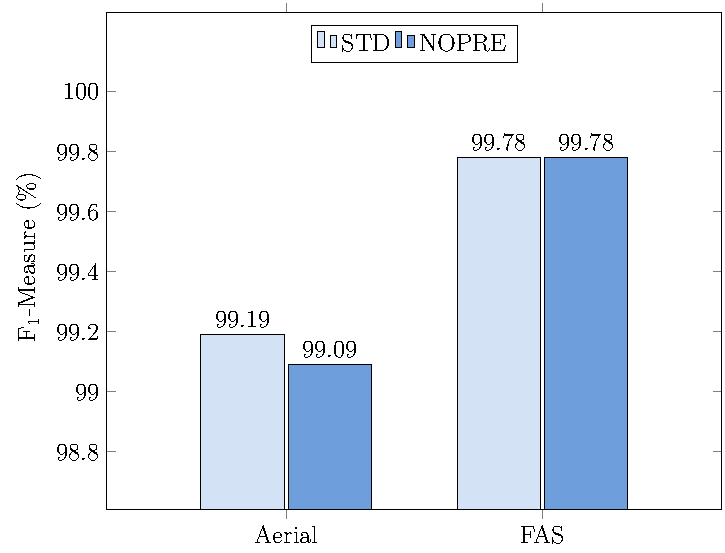
\includegraphics[width=0.8\textwidth]{imgs/BAR_8_bck_multicondition.pdf}
			\end{figure}
			\end{block}
		\end{column}%
	\end{columns}
\end{frame}

\section{Unsupervised Approach}

\subsection{OCSVM}
\subsection{End-To-End CNN-AE}
	\begin{frame}[t]{Unsupervised Approach}
		%	\textbf{An End-To-End Unsupervised Approach employing
		%		CNN Autoencoders}
		\begin{figure}
			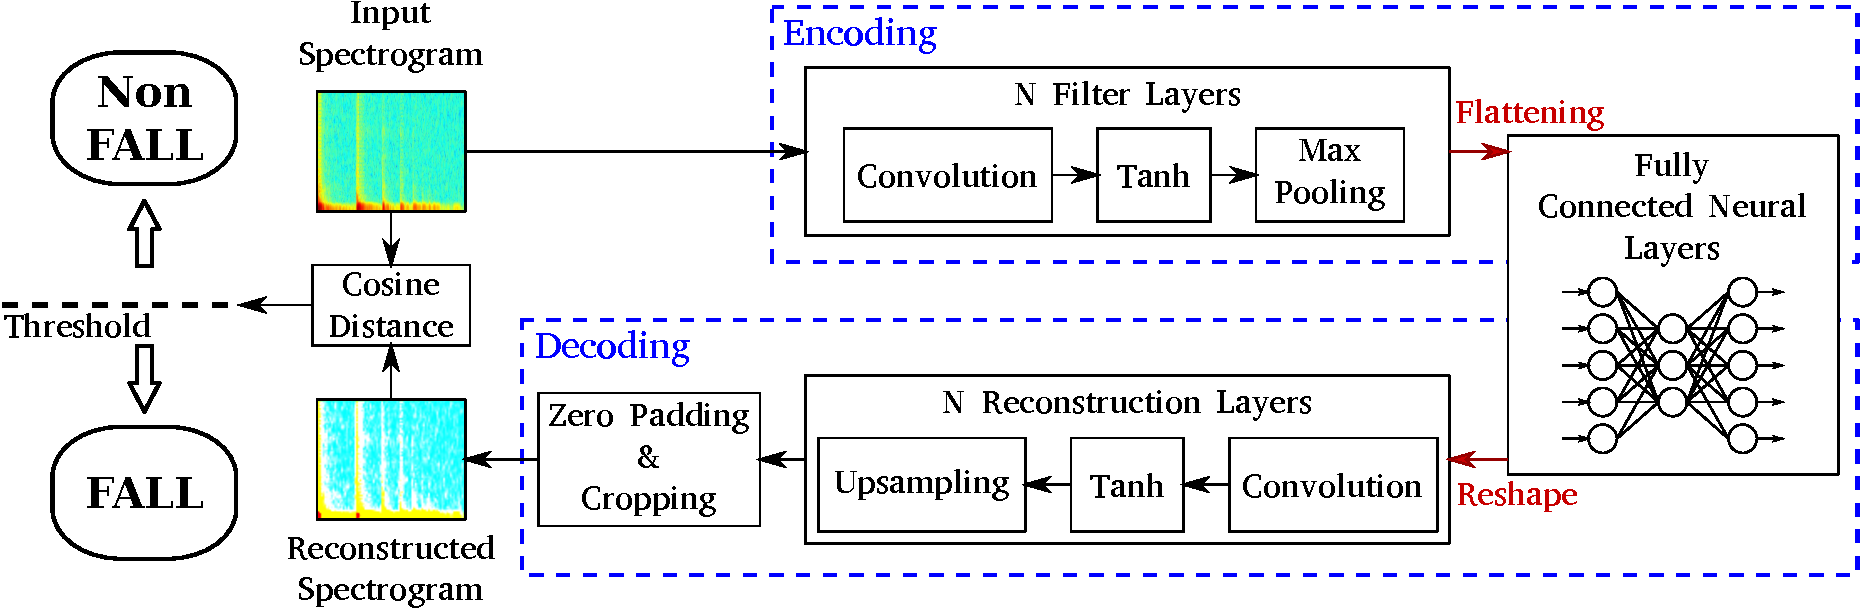
\includegraphics[width=\textwidth]{imgs/WIRN_2017_approccioComplessivo}\\

		\end{figure}
		
	\end{frame}


	\begin{frame}[t]{Results}
		%	\textbf{An End-To-End Unsupervised Approach employing
		%	CNN Autoencoders}\\
		
		\begin{columns}[T] % align columns
			\begin{column}{.4\textwidth}
				\vspace{1cm}
				\begin{itemize}
					\item Trained with background sounds only
					\item Tested with:
					\begin{itemize}
						\item background 
						\item human fall
					\end{itemize}
				\end{itemize}	
			\end{column}%
			\begin{column}{.6\textwidth}
				\begin{figure}
					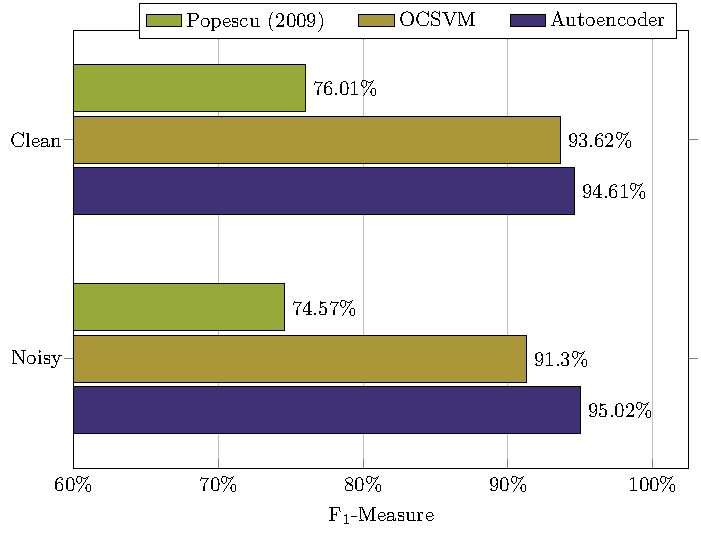
\includegraphics[width=\textwidth]{imgs/wirn_2017_results}\\
					
				\end{figure}
				
			\end{column}%
		\end{columns}
	\end{frame}
\section{Weakly-supervised Approach}
\subsection{OCSVM + Template Matching User-Aided}
	\begin{frame}[t]{OCSVM user-aided}
		%	\centerin
		%	\textbf{A Combined One-Class SVM and Template
		%		Matching Classifier in a Semi-unsupervised Framework}\\
		\begin{columns}[T] % align columns
			\begin{column}{.4\textwidth}
				%	\includegraphics[width=\textwidth]{Images/CIN_2016_approccioComplessivo}
				\begin{itemize}
					\item 1� Stage: OCSVM
					\begin{itemize}
						\item trained with non-fall event
					\end{itemize}
					\item 2� Stage: template matching 
					\begin{itemize}
						\item based on Euclidean Distance 
					\end{itemize}
					\item Final decision
					\begin{itemize}
						\item user-aided: false positive report
					\end{itemize}
				\end{itemize}
			\end{column}%
			
			\begin{column}{.6\textwidth}
				\vspace{-.2cm}
				\centering
				%			 Euclidean Distance 
				%			Threshold decision:
				\begin{figure}
					%				\includegraphics[width=\textwidth]{Images/CIN_2016_distribuzione_Caso2_Clean}\\
					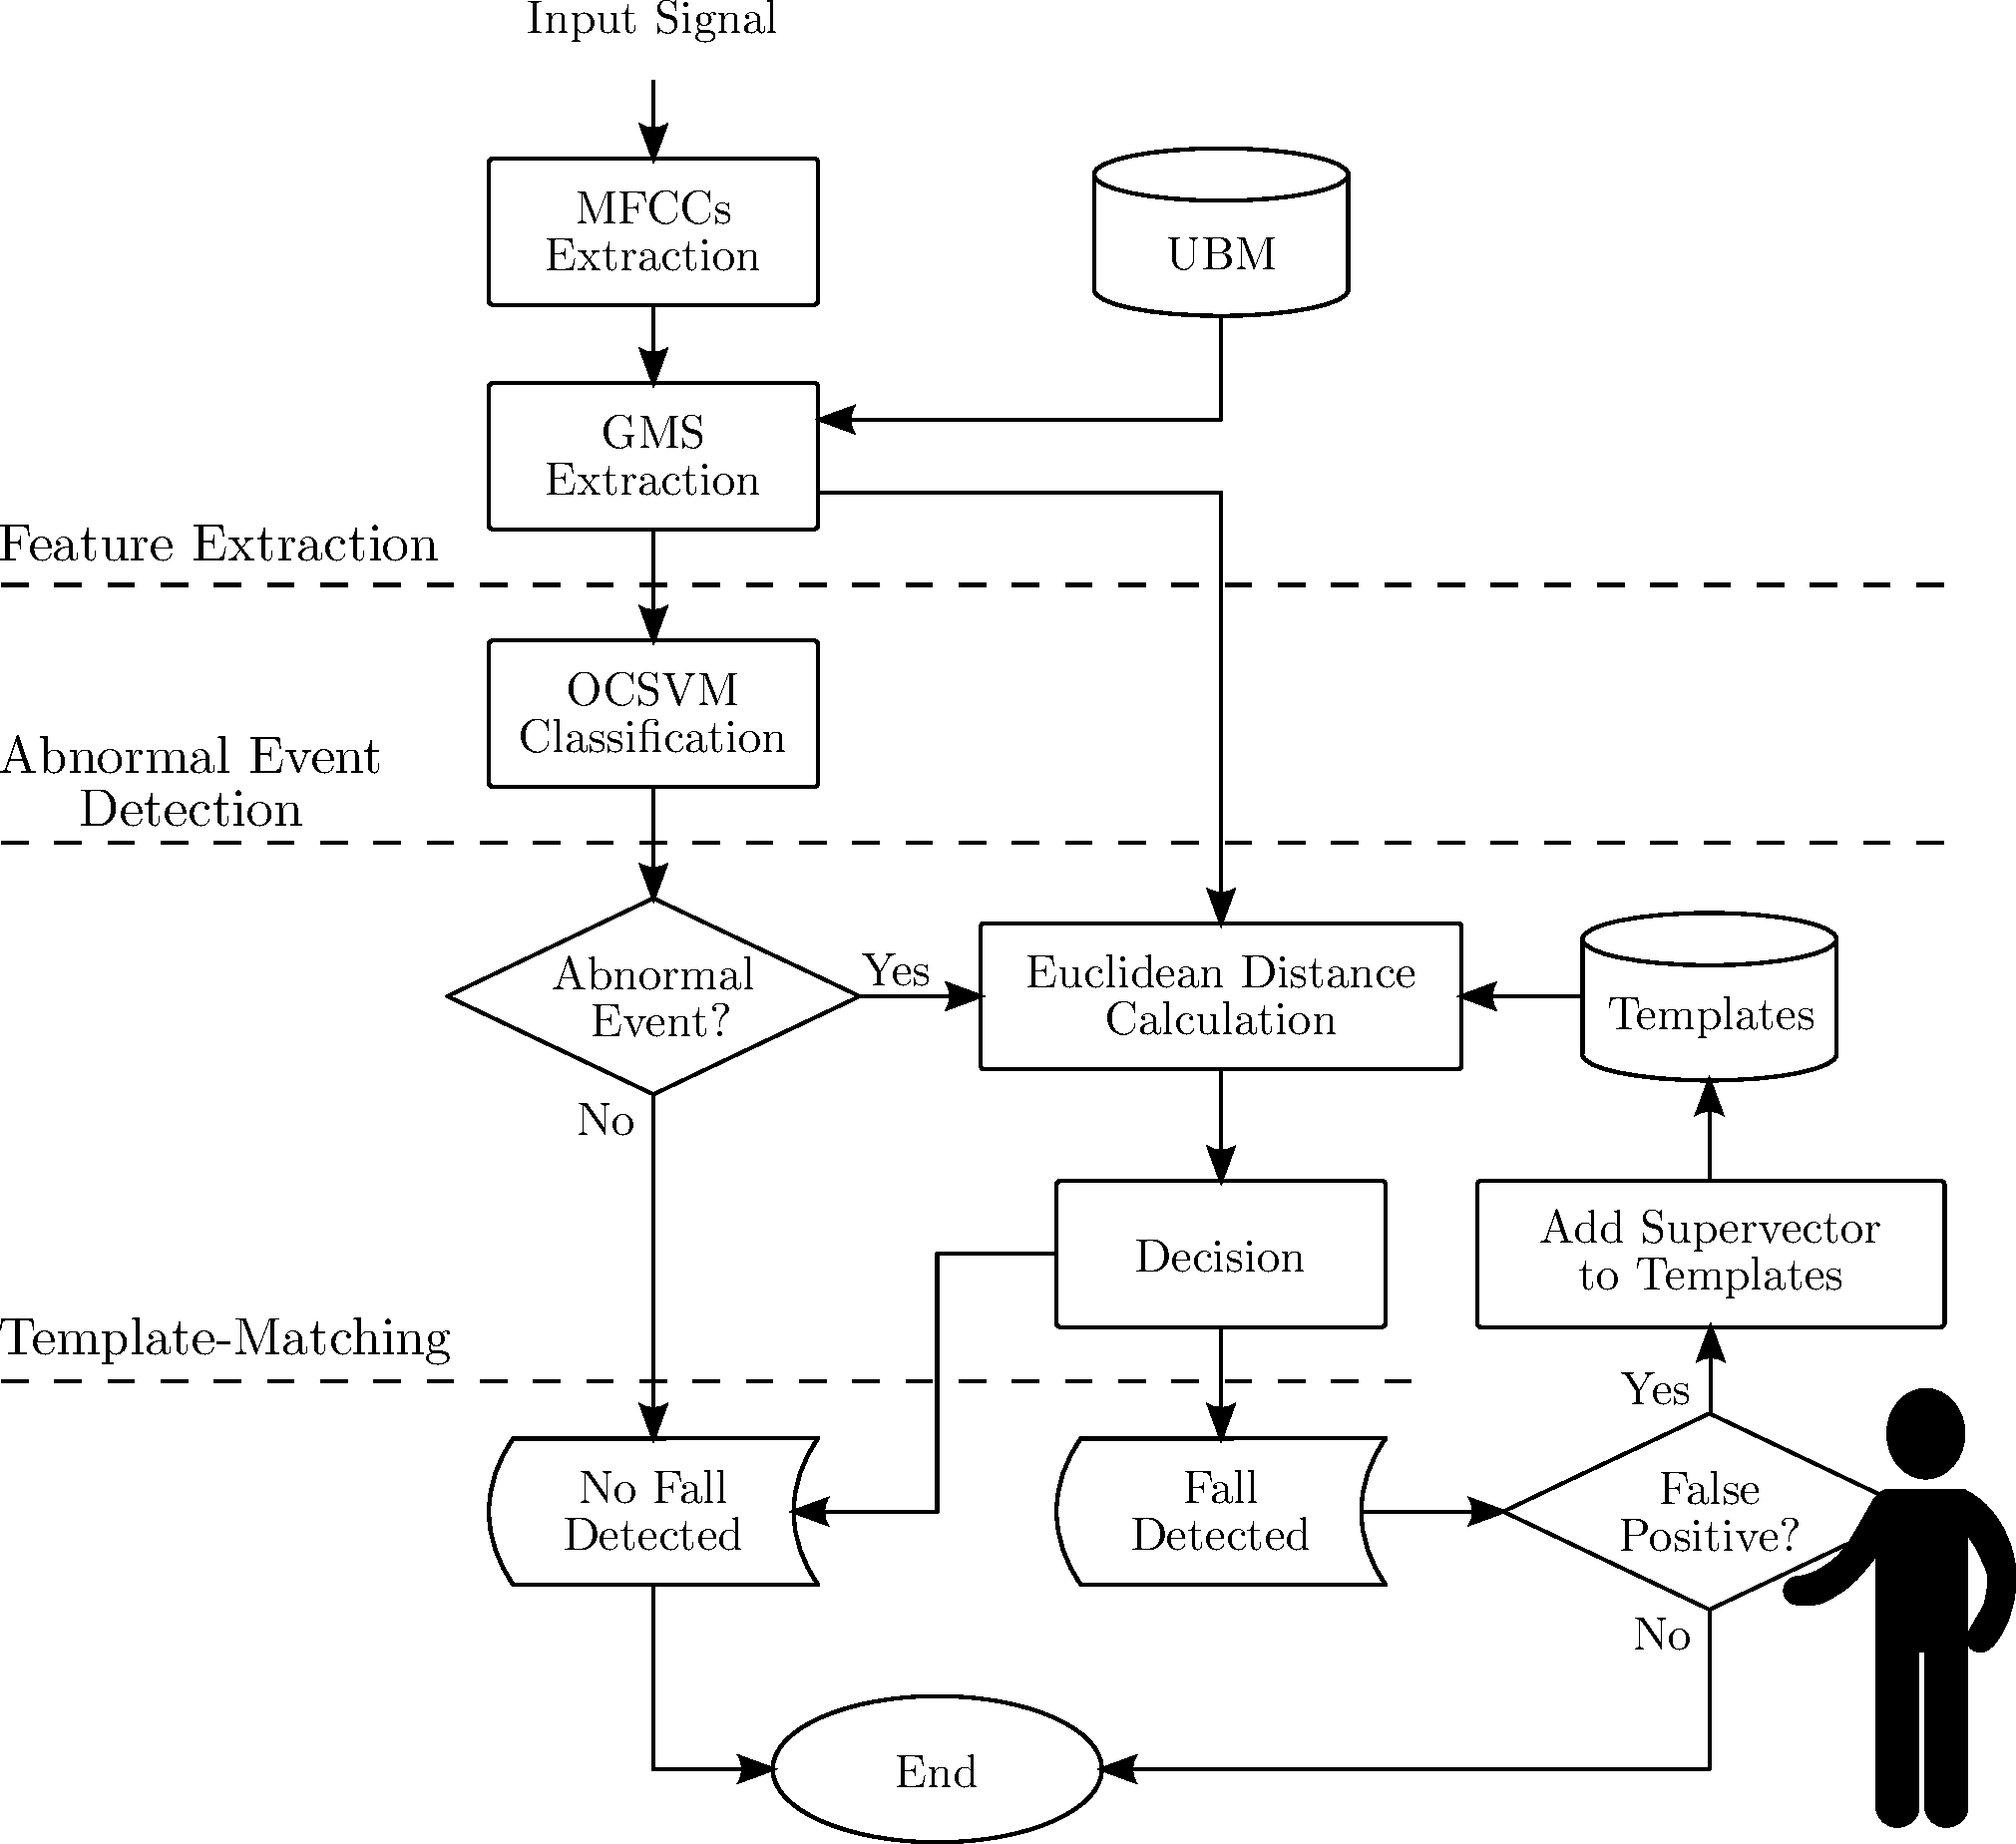
\includegraphics[width=\textwidth]{imgs/approccioComplessivo_cin}\\
				\end{figure}
				{\footnotesize 
					
					%			$	D(ValidationSet ; Templates) $
					%				$	D_{min}(V ; T) $
				}
				\vspace{.5cm}
			\end{column}%
		\end{columns}
		
	\end{frame}
	\begin{frame}[t]{Results}
		%		\textbf{A Combined One-Class SVM and Template
		%		Matching Classifier in a Semi-unsupervised Framework}\\
		\vfill
		\begin{columns}[T] % align columns
			\begin{column}{.5\textwidth}
				\begin{block}{Clean condition}

					\begin{figure}
%						\caption{Clean condition}
						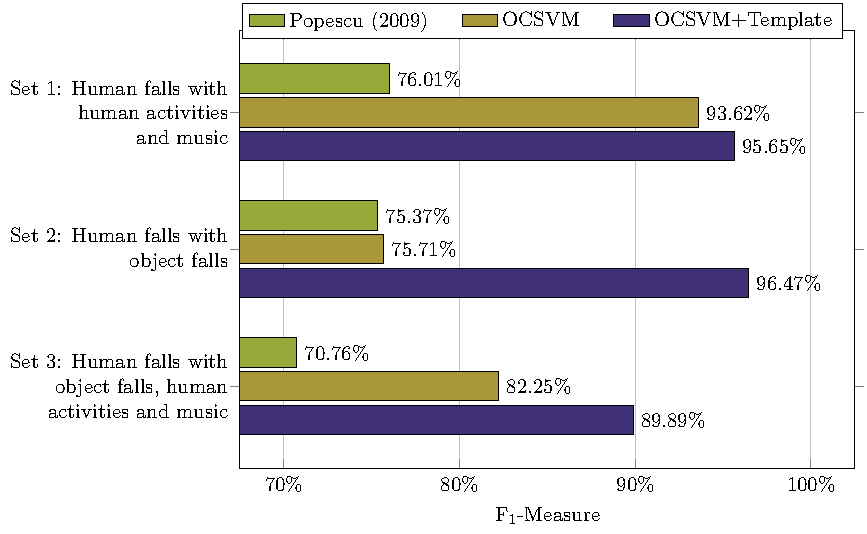
\includegraphics[width=\textwidth]{imgs/CIN_2016_res_clean}
					\end{figure}
				\end{block}
			\end{column}%
			
			\begin{column}{.5\textwidth}
				
				\begin{block}{Noisy condition}

					\begin{figure}
%						\caption{Clean condition}
						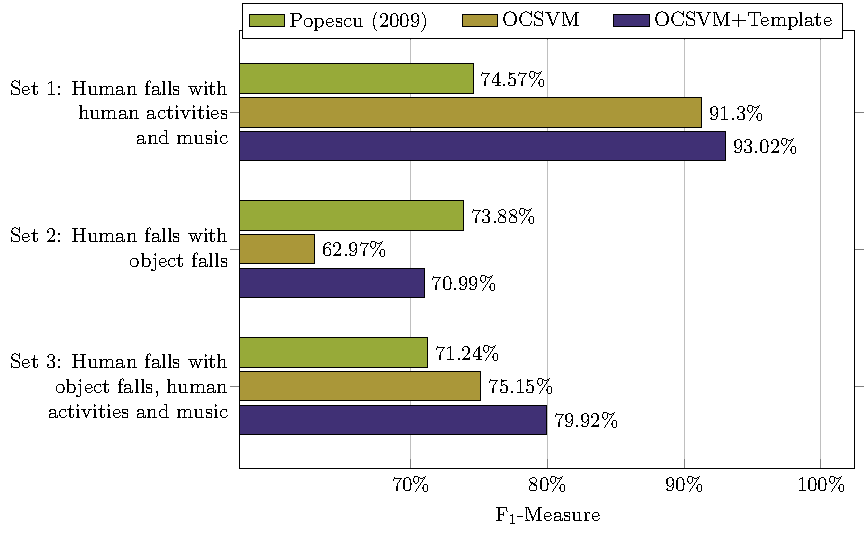
\includegraphics[width=\textwidth]{imgs/CIN_2016_res_noisy}
					\end{figure}
				\end{block}
			\end{column}%
		\end{columns}

		\vfill
	\end{frame}
\subsection{Few-shot Siamese Neural Networks}
	\begin{frame}[t]{Few-shot Siamese Neural Networks}
		%	\textbf{Few-shot Siamese Neural Networks employing Audio features
		%		for Human-Fall Detection}
		\begin{figure}
			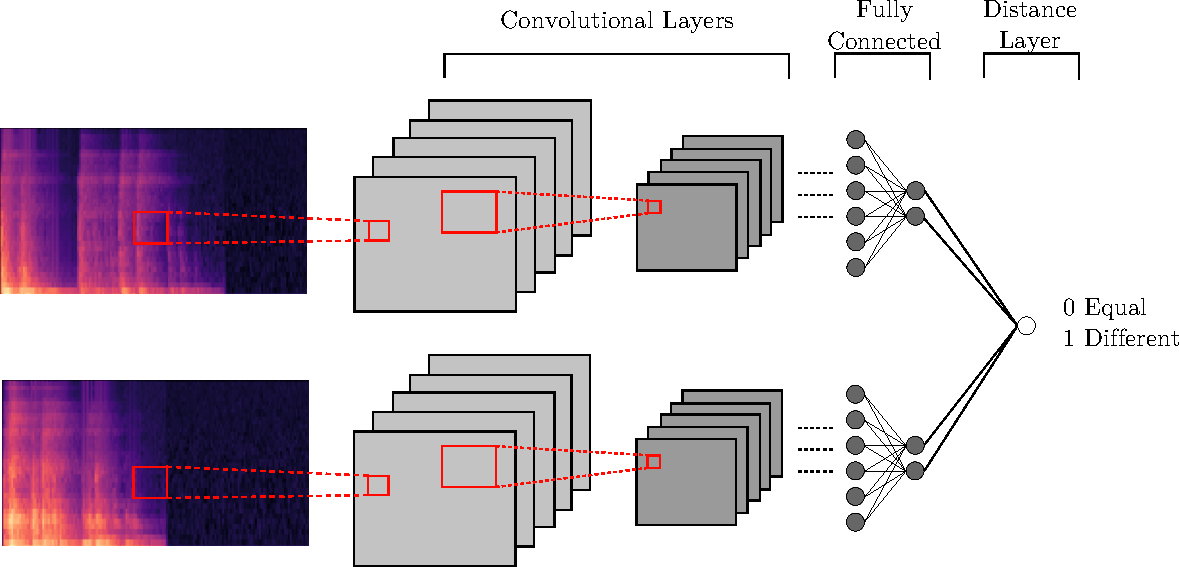
\includegraphics[width=0.8\textwidth]{imgs/prai2018_approach}\\
			
		\end{figure}
		\centering
		$Loss = (1 - Y)\frac{1}{2}(E_w)^2 + (Y)\frac{1}{2}\{(max(0, m - E_w)\}^2 $
	\end{frame}

	\begin{frame}[t]{Training Phase}
		
		Consider $X_1$, $X_2$ as a pair of two
		input samples.
		\begin{block}{Euclidean Distance}
			\begin{equation}
			E_w = \norm{S_e (X_1) - S_e (X_2)}.
			\end{equation}
			\center with  $S_e(X1)$ and $S_e(X2)$
			the mappings performed by the network 
		\end{block}	
		\vspace{0.5cm}
		The label for training a SNN are built as follows:
		\begin{itemize}
			\item Positive examples labelled as 0: pair of input samples belonging to the same fall event class
			\item Negative examples labelled as 1: pair of input samples not belonging to the same fall event class
		\end{itemize}
		%			\begin{block}{Loss Function}
		%				\begin{equation}\label{eq:loss}
		%				Loss = (1 - Y)\frac{1}{2}(E_w)^2 + (Y)\frac{1}{2}\{(max(0, m - E_w)\}^2 .
		%				\end{equation}
		%				\center with 
		%			\end{block}
		
	\end{frame}
	\begin{frame}{Results}

		\begin{columns}[T] % align columns
			\begin{column}{.4\textwidth}
				\vspace{1cm}
				\begin{itemize}
					\item Data augmentation
					\item Trained:
					\begin{itemize}
						\item objects fall
						\item 1 human fall
					\end{itemize}
					\item Tested with:
					\begin{itemize}
						\item objects fall 
						\item human fall
					\end{itemize}
				\end{itemize}	
			\end{column}%
			\begin{column}{.6\textwidth}
				\begin{figure}
					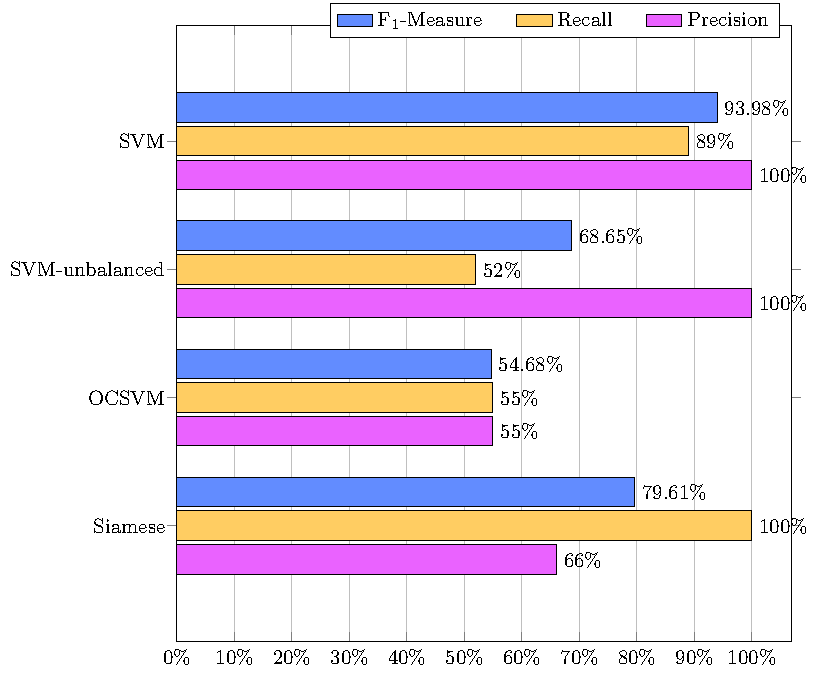
\includegraphics[width=\textwidth]{imgs/prai2018_results_f1}\\
					
				\end{figure}
				
			\end{column}%
		\end{columns}
	\end{frame}
\subsection{OneShot Siamese Autoencoders}	
	\begin{frame}[t]{OneShot Siamese Autoencoders}
		%	\textbf{Robust Feature Representation by using Siamese Autoencoders for One-Shot Audio Fall Detection}
		\begin{figure}
			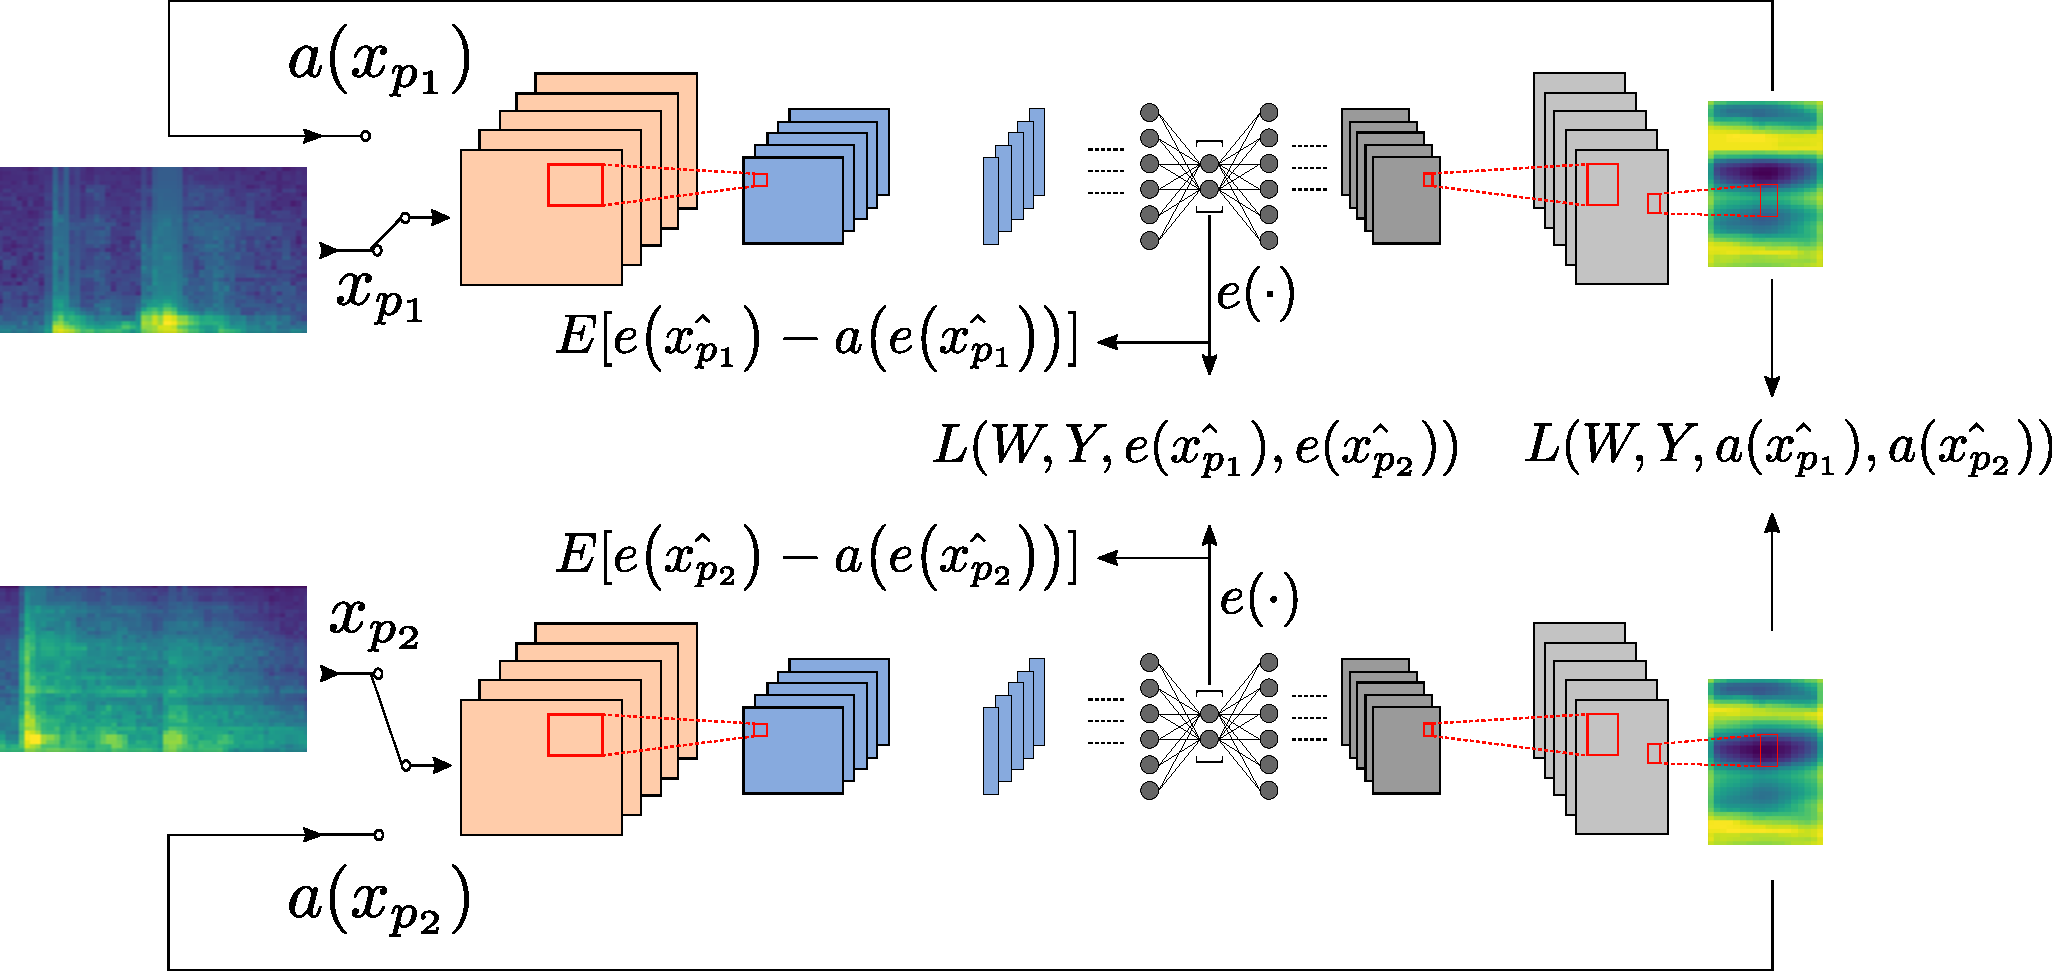
\includegraphics[width=0.9\textwidth]{imgs/SCANN_approach.pdf}\\
		\end{figure}
		
	\end{frame}
	\begin{frame}[t]{Training procedure}
		
		\begin{itemize}
			\item Contrastive loss of latent spaces
			\item Contrastive loss of reconstructions
			\item Recostruction loss (mse) of latent spaces
			\item To exploit the few human fall samples available a smart selection of the train pairs has been done:
			\begin{itemize}
				\item Neither the real falls nor the simulated falls were coupled with the falls of the objects
				\item Simulated and real falls were coupled together
			\end{itemize}
			\item induces the network to make a transformation in the latent layer
			\item simulated human fall can be used as real human fall template in the final classifier 
			\item KNN classifier
		\end{itemize}
		
	\end{frame}
	\begin{frame}[t]{Latent space with 2 neurons}
		
		\begin{columns}[T] % align columns
			\begin{column}{.5\textwidth}
				Train set
				\begin{figure}
					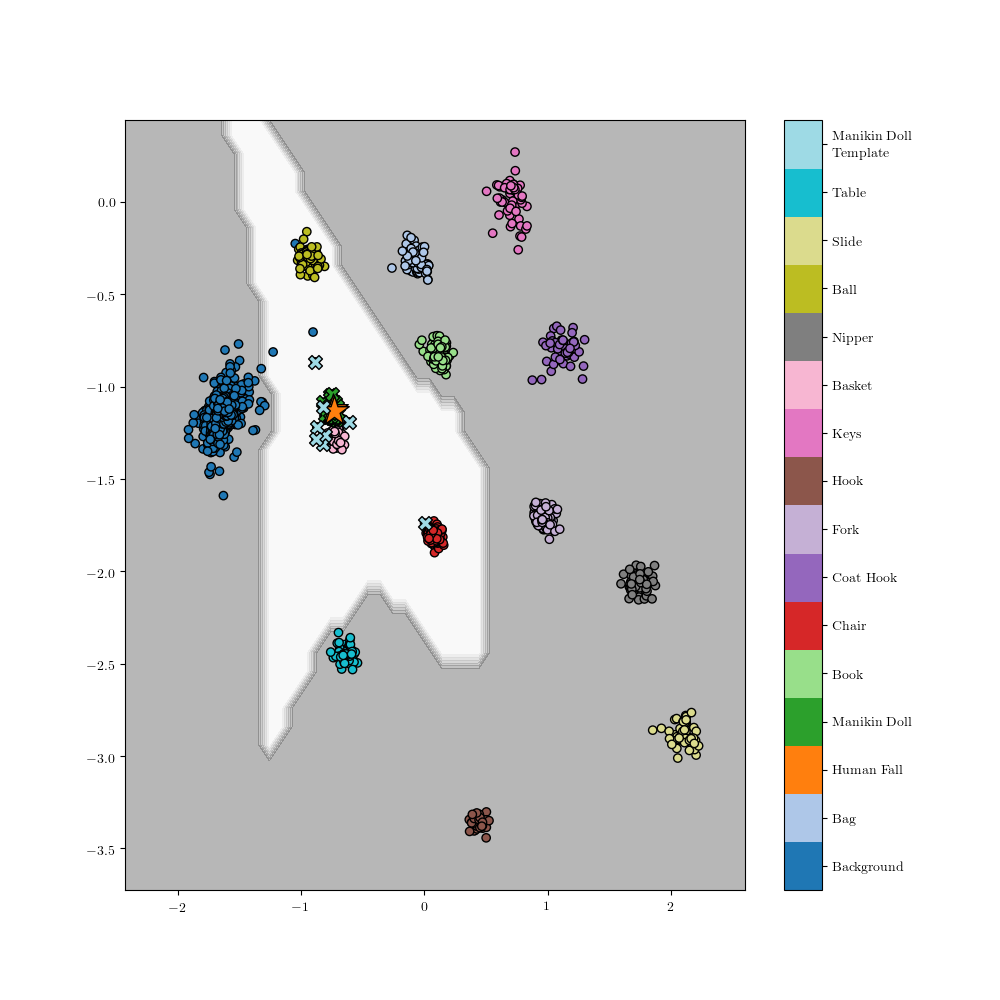
\includegraphics[width=\textwidth]{imgs/standard_3loss_term/fold_4_train}
				\end{figure}
			\end{column}%
			\begin{column}{.5\textwidth}
				Test set
				\begin{figure}
					
					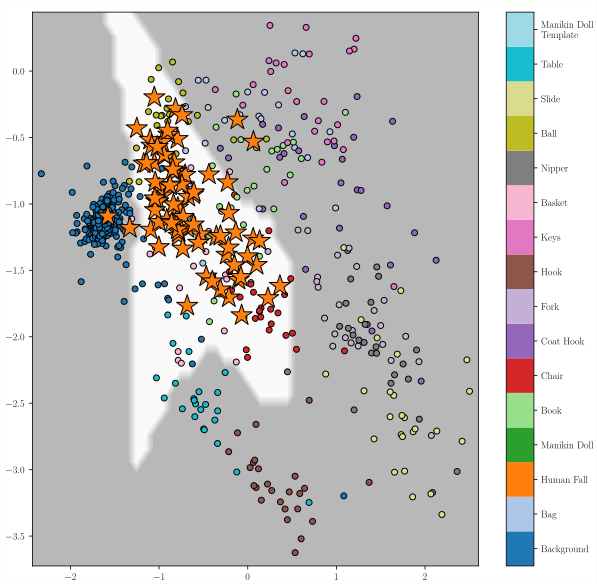
\includegraphics[width=\textwidth]{imgs/standard_3loss_term/fold_4_moquette}\\
					
				\end{figure}
				
			\end{column}%
		\end{columns}
		
	\end{frame}
	\begin{frame}[t]{Results}
		%	\textbf{Robust Feature Representation by using Siamese Autoencoders for One-Shot Audio Fall Detection}
		
		\begin{columns}[T] % align columns
			\begin{column}{.4\textwidth}
				\vspace{1cm}
				\begin{itemize}
					\item Trained (3 room):
					\begin{itemize}
						\item objects falls
						\item backgrounds
						\item manikin doll falls
						\item 1 human fall per room
					\end{itemize}
					\item Testset composed of:
					\begin{itemize}
						\item objects fall 
						\item human fall
						\item backgrounds
					\end{itemize}
				\end{itemize}	
			\end{column}%
			\begin{column}{.6\textwidth}
				\begin{figure}
					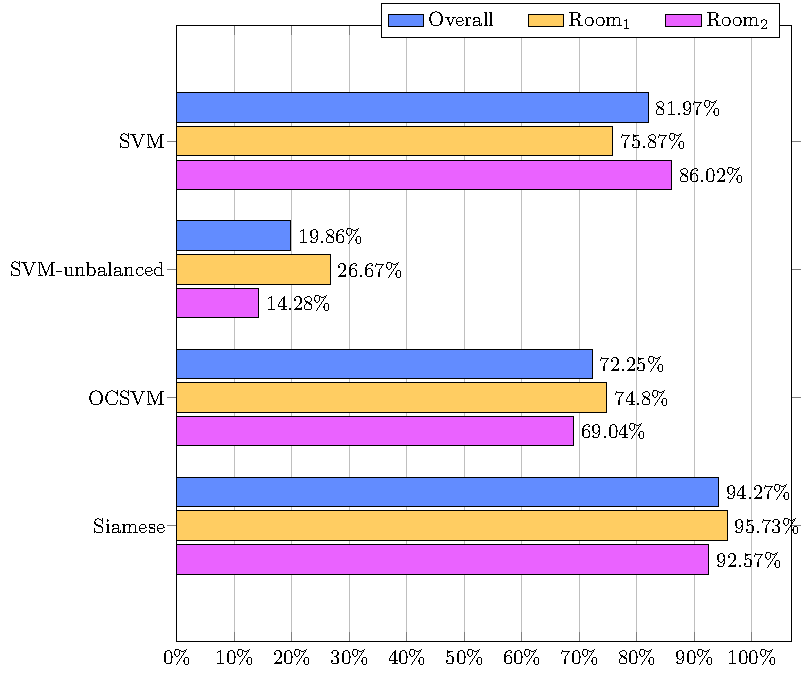
\includegraphics[width=\textwidth]{imgs/SCANN_results_f1}
				\end{figure}
				
			\end{column}%
		\end{columns}
	\end{frame}
\section{Other Contributions}

\begin{frame}{Audio Timbre Transfer}

\end{frame}
\section{Conclusions}
\begin{frame}{Conclusions}
	
\end{frame}





\section{References}
\begin{frame}[allowframebreaks]
	\scriptsize
	\frametitle{References} 
	\nocite{*} 
	\bibliographystyle{IEEEbib} 
	\bibliography{mybib} 
\end{frame}

\section{Elenco Pubblicazioni}

%%%%%%%%%%%%%%%%%%%%%%%%%%%%%%%%
\begin{frame}[allowframebreaks]
\scriptsize
\frametitle{Publications List} 
\vspace{-4mm}
\textbf{International Journal}: \hfill \textit{\scriptsize[3 articles, 2 first author]}
\begin{thebibliography}{9}
\bibitem{Principi2016a}[1]
 Principi, E., Droghini, D., Squartini, S., Olivetti, P., Piazza, F.:,
\newblock ```Acoustic cues from the floor: a new approach for fall classification,'' 
\newblock {\em Expert Systems with Applications}, 2016.

\bibitem{droghiniCin1017}[2]
Droghini, D., Ferretti, D., Principi, E., Squartini, S., Piazza, F.:,
\newblock ``A combined one-class svm and template matching approach for user-aided human fall detection by means of floor acoustic features,'' \newblock {\em Computational Intelligence and Neuroscience}, 2017.
\end{thebibliography}
\vspace{2mm}
\textbf{International Journal (submitted)}: \hfill \textit{\scriptsize[1 article, 1 first author]}

\begin{thebibliography}{9}
\bibitem{droghiniSiameseFall2019}[1]
Droghini, D., Principi, E., Squartini, S., Gabrielli, L., P., Piazza.,
\newblock ``Audio Metric Learning by using Siamese
Autoencoders for One-Shot Human Fall Detection,''
\newblock {\em IEEE Transactions on Emerging Topics in Computational Intelligence}, 2018, submitted.
\end{thebibliography}

\vspace{4mm}

\textbf{International Conference}: \hfill \textit{\scriptsize[14 articles, 5 first author]}
\begin{thebibliography}{9}
\bibitem{wirn2016-fall}[1]
Droghini, D., Principi, E., Squartini, S., Olivetti, P., Piazza., F.,
\newblock ``{Human fall detection by using an innovative floor acoustic sensor},''
\newblock in {\em Proc. of WIRN}, Vietri sul Mare, Italy, May, 2016.

\bibitem{gabrielli2018deep}[2]
Gabrielli, L., Cella, E., Vesperini, F., Droghini, D., Principi, E., Squartini, S.,
\newblock ``{Deep Learning for Timbre Modification and Transfer: An Evaluation Study},'' \newblock in {\em Proc. of AES}, Milan, Italy, May, 2018.

\bibitem{droghini2018fewshot}[3]
Droghini, F., Vesperini, F., Principi, E., Squartini, S., Piazza., F.,
\newblock ``{Few-shot Siamese Neural Networks employing Audio features for Human-Fall Detection}'',
\newblock in {\em Proc. of PRAI},Kean University, Union, NJ, USA, Aug 2018.

\bibitem{vesperini2018hierarchic}[4]
Vesperini, F., Droghini, D., Principi, E., Gabrielli, L., Squartini, S.,
\newblock ``Hierarchic ConvNets Framework for Rare Sound Event Detection'', \newblock in {\em Proc. of EUSIPCO}, Rome, Italy, Sept. 2018.

\end{thebibliography}

\textbf{Others}:
\begin{thebibliography}{9}

\bibitem{vesperinihierarchic}
F.~Vesperini, D.~Droghini, D.~Ferretti, E.~Principi, L.~Gabrielli, S.~Squartini, and F.~Piazza,
\newblock ``{A hierarchic multi-scaled approach for rare sound event detection}'',
\newblock Ancona, Italy, 2017, {DCASE} {T}ech. {R}eport. {C}opyright-free.

\bibitem{gabrielli2018rima}
L.~Gabrielli, F.~Vesperini, D.~Droghini, and S.~Squartini,
\newblock ``Rima {G}lottidis: Experimenting generative raw audio synthesis for a sound installation,''
\newblock in {\em XXII Colloquium of Musical Informatics}, Udine, Italy, 20-23 Nov. 2018.

\end{thebibliography}
\end{frame}

\end{document}